%!TEX program=xelatex
\documentclass{SWRHE_Beamer}
\begin{document}

\title{气体动力学基础}
\author{李~丹}
\institute{武汉大学水利水电学院}
\date{\today}
\frame{\titlepage}

\AtBeginSection[]{
\begin{frame}[shrink]%
\frametitle{目录}
\transfade
\tableofcontents[currentsection, hideallsubsections]
\end{frame}
}

\section{气体基本概念}
%\section{气体基本概念}
\subsection{状态方程}
\begin{frame}{完全气体状态方程}
  \only<1>{
    \begin{description}
      \item[\color{blue}理想气体] 假想的没有粘滞性的流体,即$\mu=0$
      \item[\color{blue}完全气体] 假想气体,仅考虑分子热运动,忽略分子间内聚力与分子体积
    \end{description}
  }
  完全气体状态方程——形式1:
  \begin{equation*}
    pV = nR_{u}T
  \end{equation*}
  \only<1>{
    \begin{itemize}
      \item $p$:气体绝对压强
      \item $V$:气体体积
      \item $n$:气体摩尔数
      \item $R_{u}=8.314\mathrm{J/(mol\cdot K)}$:通用气体常数
      \item $T$:气体绝对温度
    \end{itemize}
  }
  \uncover<2>{
    \vspace*{-1em}
    \begin{equation*}
      p
      =
      \frac{nM}{V}
      \frac{R_{u}}{M}T
      =
      \frac{m}{V}
      RT
      =
      \rho RT
    \end{equation*}
    完全气体状态方程——形式2:
    \begin{equation*}
      \frac{p}{\rho}
      =
      RT
    \end{equation*}
    \begin{equation*}
      p\bar{v}=RT
    \end{equation*}
    \vspace*{-0.5em}
    \begin{itemize}
      \item $M$:气体分子摩尔质量
      \item $m=nM$:气体质量
      \item $\displaystyle R=\frac{R_{u}}{M}$:气体常数,单位为$\mathrm{J/(kg\cdot K)}$
      \item $\bar{v}$:比体积$\bar{v}=1/\rho$
    \end{itemize}
  }
\end{frame}


\subsection{热动力性质}
\begin{frame}{比热、焓、熵}
  \begin{itemize}[<+-|alert@+>]
    \item 单位质量的物质温度每升高一度所需的热量为{\color{blue}比热\color{red}$c$}。
      %\item 气体比热取决于伴随温度变化的过程
    \item 温度变化过程中体积保持不变的比热为{\color{blue}定容比热
      \color{red}$\displaystyle c_{v} = \frac{\mathrm{d}e}{\mathrm{d}T}$},
      $e=c_{v}T$
    \item 温度变化过程中压强保持不变的比热为{\color{blue}定压比热
      \color{red}$\displaystyle c_{p}=\frac{\mathrm{d}h}{\mathrm{d}T} $},
      $h=c_{p}T$
    \item {\color{blue}焓\color{red}$h= e + p\bar{v} = e + RT$},$\displaystyle
      \frac{\mathrm{d} h}{\mathrm{d} T}
      =
      \frac{\mathrm{d} e + \mathrm{d}(RT)}{\mathrm{d} T}
      =
      \frac{\mathrm{d} e}{\mathrm{d} T}
      +
      R
      $
      \begin{equation*}
        c_{p} - c_{v} = R
      \end{equation*}
    \item {\color{blue}比热比\color{red}$\displaystyle \gamma=\frac{c_{p}}{c_{v}}$}。对完全气体绝热过程,$\gamma$等于绝热指数$K$
    \item $\displaystyle c_{p} = \frac{\gamma}{\gamma-1}R$,$\displaystyle c_{v}=\frac{1}{\gamma-1}R$
    \item {\color{blue}熵\color{red}$\displaystyle s = c_{v}\ln{\frac{p}{\rho^{\gamma}}}$}
  \end{itemize}
\end{frame}

\subsection{过程方程}
\begin{frame}{等熵过程}
  \begin{itemize}
    \item 等熵过程方程
      \begin{equation*}
        \frac{p}{\rho^{\gamma}}
        =
        p\bar{v}^{\gamma}
        =
        \mathrm{C}
      \end{equation*}
    \item 初、终态参数间关系
      \begin{equation*}
        \begin{aligned}
          \frac{p_{2}}{p_{1}}
           &=
           \left(\frac{\rho_{2}}{\rho_{1}}\right)^{\gamma}
           \\
           \frac{p_{2}}{p_{1}}
           &=
           \left(\frac{\bar{v}_{1}}{\bar{v}_{2}}\right)^{\gamma}
           \\
           \frac{T_{2}}{T_{1}}
           &=
           \left(\frac{\rho_{2}}{\rho_{1}}\right)^{\gamma-1}
           \\
           \frac{T_{2}}{T_{1}}
           &=
           \left(\frac{\bar{v}_{1}}{\bar{v}_{2}}\right)^{\gamma-1}
           \\
           \frac{T_{2}}{T_{1}}
           &=
           \left(\frac{p_{2}}{p_{1}}\right)^{\frac{\gamma-1}{\gamma}}
        \end{aligned}
      \end{equation*}
  \end{itemize}
\end{frame}

\subsection{气体压缩性}
\begin{frame}{体积弹性模量}
  \vspace*{-0.5em}
  \begin{definition}[体积弹性模量]
    \begin{equation*}
      E_{v}
      =
      -\frac{\mathrm{d}p}{\mathrm{d}V/V}
      \only<5>{
        =
        \frac{\mathrm{d}p}{\mathrm{d}\rho/\rho}
      }
    \end{equation*}
    \vspace*{-1em}
    \begin{itemize}
      \item $\mathrm{d}p$:压强变化量
      \item $\mathrm{d}V$:体积变化量
      \item $V$:初始体积
      \item 上式中负号是因为当$\mathrm{d}p$为正时,$\mathrm{d}V$为负
      \item $E_{v}$越大,气体越难被压缩;$E_{v}$越小,气体越易被压缩;
    \end{itemize}
  \end{definition}
  \vspace*{-1.5em}
  \begin{equation*}
    \only<2->{
      m = \rho V
    }
  \end{equation*}
  \begin{equation*}
    \only<3->{
      \mathrm{d}m
      =
      \rho\mathrm{d}V
      +
      V\mathrm{d}\rho
      =
      0
    }
  \end{equation*}
  \begin{equation*}
    \only<4->{
      \frac{\mathrm{d}\rho}{\rho}
      =
      -\frac{\mathrm{d}V}{V}
    }
  \end{equation*}
\end{frame}

\begin{frame}{体积弹性模量——续}
  对完全气体等温过程:
  \begin{equation*}
    \frac{\mathrm{d}p}{\mathrm{d}\rho}
    =
    RT
  \end{equation*}
  \begin{equation*}
    E_{v}
    =
    \rho\frac{\mathrm{d}p}{\mathrm{d}\rho}
    =
    \rho RT
    =
    p
  \end{equation*}
  对绝热过程:
  \begin{equation*}
    \frac{p}{\rho^{\gamma}} = \mathrm{C}
  \end{equation*}
  \begin{equation*}
    \mathrm{d}p
    =
    \mathrm{C}\gamma \rho^{\gamma-1}\mathrm{d}\rho
    =
    \frac{p}{\rho^{\gamma}}\gamma \rho^{\gamma-1}\mathrm{d}\rho
  \end{equation*}
  \begin{equation*}
    \frac{\mathrm{d}p}{\mathrm{d}\rho}
    =
    \gamma\frac{p}{\rho}
    =
    \gamma RT
  \end{equation*}
  \begin{equation*}
    E_{v}
    =
    \rho\frac{\mathrm{d}p}{\mathrm{d}\rho}
    =
    \gamma\rho RT
    =\gamma p
  \end{equation*}

\end{frame}


\section{气体动力学基本方程组}
%\section{气体动力学基本方程组}
\subsection{实际流体运动基本方程组}
\begin{frame}{纳维-斯托克斯方程组}
  \vspace*{-1.5em}
  \begin{equation*}
    \left\{
      \begin{aligned}
      &\frac{\partial \rho}{\partial t}
      +
      \frac{\partial (\rho u_{x})}{\partial x}
      +
      \frac{\partial (\rho u_{y})}{\partial y}
      +
      \frac{\partial (\rho u_{z})}{\partial z}
      =
      0
      \\
      &
      \frac{\partial u_{x}}{\partial t}
      +
      u_{x}\frac{\partial u_{x}}{\partial x}
      +
      u_{y}\frac{\partial u_{x}}{\partial y}
      +
      u_{z}\frac{\partial u_{x}}{\partial z}
      =
      f_{x}
      -
      \frac{1}{\rho}\frac{\partial p}{\partial x}
      +
      \nu
      \left(
        \frac{\partial^{2} u_{x}}{\partial x^{2}}
        +
        \frac{\partial^{2} u_{x}}{\partial y^{2}}
        +
        \frac{\partial^{2} u_{x}}{\partial z^{2}}
      \right)
      \\
      &
      \frac{\partial u_{y}}{\partial t}
      +
      u_{x}\frac{\partial u_{y}}{\partial x}
      +
      u_{y}\frac{\partial u_{y}}{\partial y}
      +
      u_{z}\frac{\partial u_{y}}{\partial z}
      =
      f_{y}
      -
      \frac{1}{\rho}\frac{\partial p}{\partial y}
      +
      \nu
      \left(
        \frac{\partial^{2} u_{y}}{\partial x^{2}}
        +
        \frac{\partial^{2} u_{y}}{\partial y^{2}}
        +
        \frac{\partial^{2} u_{y}}{\partial z^{2}}
      \right)
      \\
      &
      \frac{\partial u_{z}}{\partial t}
      +
      u_{x}\frac{\partial u_{z}}{\partial x}
      +
      u_{y}\frac{\partial u_{z}}{\partial y}
      +
      u_{z}\frac{\partial u_{z}}{\partial z}
      =
      f_{z}
      -
      \frac{1}{\rho}\frac{\partial p}{\partial z}
      +
      \nu
      \left(
        \frac{\partial^{2} u_{z}}{\partial x^{2}}
        +
        \frac{\partial^{2} u_{z}}{\partial y^{2}}
        +
        \frac{\partial^{2} u_{z}}{\partial z^{2}}
      \right)
      \end{aligned}
      \right.
  \end{equation*}
  \begin{equation*}
    \left\{
      \begin{aligned}
    &\frac{\partial \rho}{\partial t}
    +
    \nabla\cdot(\rho\bm{u})
    =
    0
    \\
    &\frac{\partial \bm{u}}{\partial t}
    +
    \bm{u}\cdot \nabla\bm{u}
    =
    \bm{f}
    -
    \frac{1}{\rho}\nabla p
    +
    \nu\nabla^{2}\bm{u}
      \end{aligned}
      \right.
  \end{equation*}
\end{frame}

\subsection{气体动力学基本方程组}
\begin{frame}{气体动力学基本方程组}
  \vspace*{-1em}
  \begin{equation*}
    \left\{
      \begin{aligned}
    &\frac{\partial \rho}{\partial t}
    +
    \nabla\cdot(\rho\bm{u})
    =
    0
    \\
    &
    \frac{\mathrm{d} \bm{u}}{\mathrm{d} t}
    =
    \frac{\partial \bm{u}}{\partial t}
    +
    \bm{u}\cdot \nabla\bm{u}
    =
    \only<1-4>{
    \bm{f}
  }
    -
    \frac{1}{\rho}\nabla p
    \only<1-2>{
    +
    \nu\nabla^{2}\bm{u}
  }
  \only<7-10>{
  \\
    &
    \frac{\mathrm{d} s}{\mathrm{d} t}
    =
    0
  }
  \only<11->{
  \\
    &
    \frac{p}{\rho^{\gamma}}
    =
    \mathrm{C}
  }
    \only<10-11>{
    \\
    &
    p = \rho RT
  }
      \end{aligned}
      \right.
  \end{equation*}
  \uncover<2->{
  \begin{block}{气体假定条件}
  \begin{enumerate}
    \item<2-|alert@2> 忽略粘性的作用,将气体看作理想流体
    \item<4-|alert@4> 忽略质量力的作用
    \item<6-|alert@6> 忽略热传导的作用,将运动过程看作绝热过程
    \item<9-|alert@9> 假设气体是完全气体,且比热是常数
  \end{enumerate}
  \end{block}
}
\end{frame}


\section{声速与马赫数}
%\section{声速与马赫数}
\subsection{微弱扰动的一维传播}
\begin{frame}{微弱扰动的一维传播过程}
  \begin{figure}
    \begin{tikzpicture}
      \begin{scope}
      \draw[thick] (0,0) -- (4,0);
      \draw[thick] (0,1.5) -- (4,1.5);
      \foreach \p in 
    {0.1, 0.2, 0.3, 0.4, 0.5, 0.6, 0.7, 0.8, 0.9, 1.0,
     1.1, 1.2, 1.3, 1.4, 1.5, 1.6, 1.7, 1.8, 1.9, 2.0,
     2.1, 2.2, 2.3, 2.4, 2.5, 2.6, 2.7, 2.8, 2.9, 3.0,
     3.1, 3.2, 3.3, 3.4, 3.5, 3.6, 3.7, 3.8, 3.9}
     {
      \draw[thin] (\p, 0) -- ++(-45:0.1);
      \draw[thin] (\p, 1.5) -- ++(45:0.1);
     }
     \draw[dashed,thin] (2,0) node[below]{$n$} -- (2,1.5) node[above]{$m$};
     \draw[-latex,thick] (2,0.75) -- node[midway,above]{$c$} ++(1,0);
     \node at (3.5, 1.2) {$p_{1}$};
     \node at (3.5, 0.8) {$\rho_{1}$};
     \node at (3.5, 0.4) {$T_{1}$};
     \node at (1.5, 1.2) {$p_{2}$};
     \node at (1.5, 0.8) {$\rho_{2}$};
     \node at (1.5, 0.4) {$T_{2}$};

     \draw[thin] (0.8,0) -- (0.8,1.5);
     \draw[thin] (1.0,0) -- (1.0,1.5);
     \draw[thick,fill=black] (0.6,0.6) -- (0.8, 0.6) -- (0.8, 0.9) -- (0.6,0.9) -- cycle;
     \draw[-latex,thick] (0.1,0.75) -- node[midway,above]{$\mathrm{d}v$}(0.6,0.75);
   \end{scope}

     \begin{scope}[yshift=-2.5cm]
       \draw[-latex, thin] (0,0) -- (4,0) node[below]{$x$};
       \draw[-latex, thin] (0,0) -- (0,2) node[left]{$p$};
       \draw[thick] (0,1.5) -- node[midway,above]{$p_{2}$} (2,1.5);
       \draw[thick] (2,1) -- node[midway,above]{$p_{1}$} (4,1);
       \draw[thin,dashed] (2,0) -- (2,2);
     \end{scope}

     \begin{scope}[yshift=-4cm]
       \draw[-latex, thin] (0,0) -- (4,0) node[below]{$x$};
       \draw[-latex, thin] (0,-0.6) -- (0,1) node[left]{$v$};
       \draw[thick] (0,0.5) -- node[midway,above]{$\mathrm{d}v$} (2,.5);
       \draw[thin,dashed] (2,-0.6) -- (2,1);
       \node at (2,-0.6) [anchor=north]{(a)活塞向右移动,压缩波};
     \end{scope}


     \begin{scope}[xshift=6cm]
      \draw[thick] (0,0) -- (4,0);
      \draw[thick] (0,1.5) -- (4,1.5);
      \foreach \p in 
    {0.1, 0.2, 0.3, 0.4, 0.5, 0.6, 0.7, 0.8, 0.9, 1.0,
     1.1, 1.2, 1.3, 1.4, 1.5, 1.6, 1.7, 1.8, 1.9, 2.0,
     2.1, 2.2, 2.3, 2.4, 2.5, 2.6, 2.7, 2.8, 2.9, 3.0,
     3.1, 3.2, 3.3, 3.4, 3.5, 3.6, 3.7, 3.8, 3.9}
     {
      \draw[thin] (\p, 0) -- ++(-45:0.1);
      \draw[thin] (\p, 1.5) -- ++(45:0.1);
     }
     \draw[dashed,thin] (2,0) node[below]{$n$} -- (2,1.5) node[above]{$m$};
     \draw[-latex,thick] (2,0.75) -- node[midway,above]{$c$} ++(1,0);
     \node at (3.5, 1.2) {$p_{1}$};
     \node at (3.5, 0.8) {$\rho_{1}$};
     \node at (3.5, 0.4) {$T_{1}$};
     \node at (1.5, 1.2) {$p_{2}$};
     \node at (1.5, 0.8) {$\rho_{2}$};
     \node at (1.5, 0.4) {$T_{2}$};

     \draw[thin] (0.8,0) -- (0.8,1.5);
     \draw[thin] (1.0,0) -- (1.0,1.5);
     \draw[thick,fill=black] (0.6,0.6) -- (0.8, 0.6) -- (0.8, 0.9) -- (0.6,0.9) -- cycle;
     \draw[-latex,thick] (0.6,0.75) -- node[midway,above]{$\mathrm{d}v$}(0.1,0.75);
   \end{scope}

     \begin{scope}[xshift=6cm,yshift=-2.5cm]
       \draw[-latex, thin] (0,0) -- (4,0) node[below]{$x$};
       \draw[-latex, thin] (0,0) -- (0,2) node[left]{$p$};
       \draw[thick] (0,1) -- node[midway,above]{$p_{2}$} (2,1);
       \draw[thick] (2,1.5) -- node[midway,above]{$p_{1}$} (4,1.5);
       \draw[thin,dashed] (2,0) -- (2,2);
     \end{scope}

     \begin{scope}[xshift=6cm,yshift=-4cm]
       \draw[-latex, thin] (0,0) -- (4,0) node[below]{$x$};
       \draw[-latex, thin] (0,-0.6) -- (0,1) node[left]{$v$};
       \draw[thick] (0,-0.5) -- node[midway,above]{$\mathrm{d}v$} (2,-0.5);
       \draw[thin,dashed] (2,-0.6) -- (2,1);
       \node at (2,-0.6) [anchor=north]{(b)活塞向左移动,膨胀波};
     \end{scope}
    \end{tikzpicture}
  \end{figure}
\end{frame}

\subsection{声速}
\begin{frame}{声速}
  \begin{itemize}
    \item 微弱扰动波在流体介质中的传播速度$c$称为声速
  \end{itemize}
  \begin{figure}
  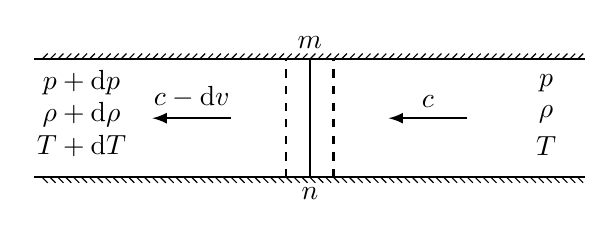
\begin{tikzpicture}
    \draw[thick] (0,0) -- (7,0);
    \draw[thick] (0,1.5) -- (7,1.5);
    \draw[thick] (3.5,0) node[anchor=north]{$n$} -- (3.5,1.5) node[anchor=south]{$m$};
    \draw[thick,dashed] (3.2,0) -- (3.2,1.5);
    \draw[thick,dashed] (3.8,0) -- (3.8,1.5);
    \draw[thick,-latex] (2.5,0.75) -- node[midway,above]{$c-\mathrm{d}v$} (1.5,0.75);
    \draw[thick,-latex] (5.5,0.75) -- node[midway,above]{$c$} (4.5,0.75);
    \node at (6.5, 1.2) {$p$};
    \node at (6.5, 0.8) {$\rho$};
    \node at (6.5, 0.4) {$T$};
    \node at (0.6, 1.2) {$p+\mathrm{d}p$};
    \node at (0.6, 0.8) {$\rho+\mathrm{d}\rho$};
    \node at (0.6, 0.4) {$T+\mathrm{d}T$};
    \foreach \p in 
    {0.1, 0.2, 0.3, 0.4, 0.5, 0.6, 0.7, 0.8, 0.9, 1.0,
     1.1, 1.2, 1.3, 1.4, 1.5, 1.6, 1.7, 1.8, 1.9, 2.0,
     2.1, 2.2, 2.3, 2.4, 2.5, 2.6, 2.7, 2.8, 2.9, 3.0,
     3.1, 3.2, 3.3, 3.4, 3.5, 3.6, 3.7, 3.8, 3.9, 4.0,
     4.1, 4.2, 4.3, 4.4, 4.5, 4.6, 4.7, 4.8, 4.9, 5.0,
     5.1, 5.2, 5.3, 5.4, 5.5, 5.6, 5.7, 5.8, 5.9, 6.0,
     6.1, 6.2, 6.3, 6.4, 6.5, 6.6, 6.7, 6.8, 6.9}
    {
      \draw[thin] (\p, 0) -- ++(-45:0.1);
      \draw[thin] (\p, 1.5) -- ++(45:0.1);
    }
  \end{tikzpicture}
  \end{figure}
  \vspace*{-0.5em}
  连续性方程:
  \vspace*{-1.3em}
  \begin{equation*}
  c\rho A\mathrm{d}t
  =
  (c-\mathrm{d}v)(\rho+\mathrm{d}\rho)A\mathrm{d}t
  \end{equation*}
  \begin{equation*}
  c\mathrm{d}\rho
  =
  \rho\mathrm{d}v
  \end{equation*}

  \vspace*{0.5em}
  动量方程:
  \vspace*{-1.8em}
  \begin{equation*}
  c\rho A\mathrm{d}t
  \frac{[(c-\mathrm{d}v)-c]}{\mathrm{d}t}
  =
  [p-(p+\mathrm{d}p)]A
  \end{equation*}
  \begin{equation*}
  c\rho\mathrm{d}v
  =
  \mathrm{d}p
  \end{equation*}
  \begin{equation*}
  c =
  \sqrt{\frac{\mathrm{d}p}{\mathrm{d}\rho}}
  \end{equation*}
\end{frame}

\begin{frame}{声速——续}
 气体为完全气体:
 \begin{equation*}
   \frac{p}{\rho^{\gamma}}
   =
   \mathrm{C}
 \end{equation*}
 \begin{equation*}
 \frac{\mathrm{d} p}{\mathrm{d} \rho}
 =
 \gamma \frac{p}{\rho}
 =
 \gamma RT
 \end{equation*}
 \begin{equation*}
 c
 =
 \sqrt{\frac{\mathrm{d}p}{\mathrm{d}\rho}}
 =
 \sqrt{\gamma\frac{p}{\rho}}
 =
 \sqrt{\gamma RT}
 \end{equation*}
 对于空气
% ($20^{\circ}\!\mathrm{C}$)
 ,$R=287\mathrm{J/kg\cdot K}$,$\gamma=1.4$
 \begin{equation*}
   c = 20.05\sqrt{T}
 \end{equation*}
 当$T=288.2\mathrm{K}=15^{\circ}\!\mathrm{C}$,$c=340.3\mathrm{m/s}$
\end{frame}

\begin{frame}{声速讨论}
  \vspace*{-1em}
  \begin{equation*}
    c = \sqrt{\gamma\frac{p}{\rho}} = \sqrt{\gamma RT}
  \end{equation*}
  \onslide<2->{
  \vspace*{-1em}
    \begin{block}{讨论}
  \begin{itemize}
    \item<2-|alert@2> 气体声速随气体的状态参数变化$c=f(p,\rho,R,T)$
    \item<3-|alert@3> 在同一流体介质中,各个点的瞬时状态参数是不同的,因而各个点的声速是不同的
    \item<4-|alert@4> 对非定常流,声速是空间和时间的函数,即$c=f(x,y,z,t)$
    \item<5-|alert@5> 对定常流,声速是空间的函数,即$c=f(x,y,z)$
    \item<6-|alert@6> 一般情况下,所提到的声速是指当地声速
    \item<7-|alert@7> 气体声速可作为判别气体压缩性标准,
      $
      \displaystyle
        E_{v}
        =
        \frac{\mathrm{d}p}{\mathrm{d}\rho/\rho}
        =
        \rho c^2
        $
        \begin{itemize}
          \item 流体可压缩性大的,$E_{v}$小,声速低
          \item 流体可压缩性小的,$E_{v}$大,声速高
        \end{itemize}
  \end{itemize}
\end{block}
}
\end{frame}

\subsection{气体流动分类}
\begin{frame}{气体流动分类、马赫数}
 \begin{block}{气体流动分类}
   \begin{enumerate}
     \item 当流速低于声速时,为亚声速流动
     \item 当流速等于声速时,为声速流动
     \item 当流速高于声速时,为超声速流动
   \end{enumerate}
 \end{block} 
 通常用无量纲数$\mathrm{Ma}$作为流动类型判别标准
 \begin{equation*}
   \mathrm{Ma}
   =
   \frac{v}{c}
 \end{equation*}
 \vspace*{-1.5em}
 \begin{block}{气体流动分类判别}
   \begin{enumerate}
     \item $v<c$或$\mathrm{Ma}<1$,为亚声速流动
     \item $v=c$或$\mathrm{Ma}=1$,为声速流动
     \item $v>c$或$\mathrm{Ma}>1$,为超声速流动
   \end{enumerate}
 \end{block} 
\end{frame}

\begin{frame}{马赫数讨论}
  \begin{equation*}
    \mathrm{Ma}
    =
    \frac{v}{c}
  \end{equation*}
  对于完全气体
  \begin{equation*}
    \mathrm{Ma}^{2}
    =
    \frac{v^{2}}{c^{2}}
    =
    \frac{v^{2}}{\gamma RT}
  \end{equation*}
  \onslide<2->{
  \begin{block}{讨论}
    \begin{itemize}
      \item<2-|alert@2> $v^{2}$表示气体宏观运动的动能大小
      \item<3-|alert@3> $T$表示气体的内能大小
      \item<4-|alert@4> $\mathrm{Ma}$表示气体宏观运动的动能与气体内能之比
      \item<5-|alert@5> $\mathrm{Ma}$小,则气体内能大而宏观动能小
      \item<6-|alert@6> $\mathrm{Ma}$大,则气体宏观动能大而内能小
    \end{itemize}
  \end{block}
}
\end{frame}

\begin{frame}{举例}
  \begin{block}{例:有一喷气式发动机,其尾部喷管出口处,气流的速度为
    $v=556\mathrm{m/s}$,气流的温度为$T=860\mathrm{K}$,气流的绝热指数
  $\gamma=1.33$,气体常数$R=287\mathrm{J/(kg\cdot K)}$,试求喷管出口处气流的声速
和马赫数,并确定流动类型。}
解:
   \begin{equation*}
   c
   =
   \sqrt{\gamma RT}
   =
   \sqrt{1.33\times 287 \times 860}
   =
   573\mathrm{m/s}
   \end{equation*} 
   \begin{equation*}
     \mathrm{Ma}
     =
     \frac{v}{c}
     =
     \frac{556}{573}
     =
     0.97 
   \end{equation*}
   $\mathrm{Ma}=0.97<1$,亚声速流动。
  \end{block}
\end{frame}


\section{微弱扰动在可压缩流体中的传播}
%\section{微弱扰动在可压缩流体中的传播}
\subsection{微弱扰动源静止不动($v=0$)}
\begin{frame}{微弱扰动源静止不动($v=0$)}
  \begin{figure}
 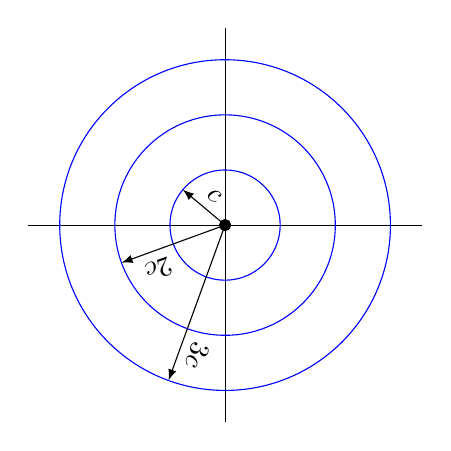
\begin{tikzpicture}
   \draw (-2.5,0) -- (2.5,0);
   \draw (0,-2.5) -- (0,2.5);
   \draw[fill] (0,0) circle (2pt);
   \uncover<2->{
     \draw[blue] (0,0) circle (0.7cm);
   \draw[-latex] (0,0) -- node[midway,above,rotate=-40]{$c$} ++(140:0.7cm);
 }
 \uncover<3->{
   \draw[blue] (0,0) circle (1.4cm);
   \draw[-latex] (0,0) -- node[pos=0.7,above,rotate=200]{$2c$} ++(200:1.4cm);
 }
 \uncover<4->{
   \draw[blue] (0,0) circle (2.1cm);
   \draw[-latex] (0,0) -- node[pos=0.8,above,rotate=250]{$3c$} ++(250:2.1cm);
 }
 \end{tikzpicture}
 \end{figure}
\end{frame}

\subsection{微弱扰动源作亚声速匀速运动($v<c$)}
\begin{frame}{微弱扰动源作亚声速匀速运动($v<c$)}
  \begin{figure}
 \begin{tikzpicture}
   \draw (-2.5,0) -- (2.5,0);
   \draw (0,-2.5) -- (0,2.5);
   \uncover<2->{
   \draw[fill] (0,0) node[anchor=north]{$0$} circle (2pt);
   \draw[fill] (-0.3,0) node[anchor=north]{$1$} circle (2pt);
 }
 \only<2>{
   \draw[blue] (0,0) circle (0.7cm);
   \draw[-latex] (0,0) -- node[pos=0.5,above,rotate=60]{$c$} ++(60:0.7cm);
 }
 \uncover<3->{
   %\draw[fill] (-0.3,0) node[anchor=north]{$1$} circle (2pt);
   \draw[fill] (-0.6,0) node[anchor=north]{$2$} circle (2pt);
 }
 \only<3>{
   \draw[blue] (0,0) circle (1.4cm);
   \draw[blue] (-0.3,0) circle (0.7cm);
   \draw[-latex] (0,0) -- node[pos=0.8,above,rotate=60]{$2c$} ++(60:1.4cm);
   \draw[-latex] (-0.3,0) -- node[pos=0.7,above,rotate=60]{$c$} ++(60:0.7cm);
 }
 \uncover<4->{
   \draw[fill] (-0.9,0) node[anchor=north]{$3$} circle (2pt);
   \draw[blue] (0,0) circle (2.1cm);
   \draw[blue] (-0.3,0) circle (1.4cm);
   \draw[blue] (-0.6,0) circle (0.7cm);
   \draw[-latex] (0,0) -- node[pos=0.8,above,rotate=60]{$3c$} ++(60:2.1cm);
   \draw[-latex] (-0.3,0) -- node[pos=0.7,above,rotate=60]{$2c$} ++(60:1.4cm);
   \draw[-latex] (-0.6,0) -- node[pos=0.5,above,rotate=60]{$c$} ++(60:.7cm);
 }
 \uncover<5->{
 \begin{scope}[xshift=5.5cm]
   \draw[fill] (0.3,0) circle (2pt);
   \draw[blue] (0.9,0) circle (2.1cm);
   \draw[blue] (0.6,0) circle (1.4cm);
   \draw[blue] (0.3,0) circle (0.7cm);
   \draw[-latex] (0.9,0)++(0:2.1) -- node[midway,anchor=south west]{$c+v$} ++(0.6,0);
   \draw[-latex] (0.9,0)++(180:2.1) -- node[midway,anchor=south east]{$c-v$} ++(180:0.4);
 \end{scope}
 }
 \end{tikzpicture}
 \end{figure}
\end{frame}

\subsection{微弱扰动源作声速匀速运动($v=c$)}
\begin{frame}{微弱扰动源作声速匀速运动($v=c$)}
  \begin{figure}
 \begin{tikzpicture}
   \draw (-2.5,0) -- (2.5,0);
   \draw (0,-2.5) -- (0,2.5);
   \uncover<2->{
   \draw[fill] (0,0) node[anchor=north]{$0$} circle (2pt);
   \draw[fill] (-0.7,0) node[anchor=north]{$1$} circle (2pt);
 }
 \only<2>{
   \draw[blue] (0,0) circle (0.7cm);
   \draw[-latex] (0,0) -- node[pos=0.5,above,rotate=60]{$c$} ++(60:0.7cm);
 }
 \uncover<3->{
   %\draw[fill] (-0.7,0) node[anchor=north]{$1$} circle (2pt);
   \draw[fill] (-1.4,0) node[anchor=north]{$2$} circle (2pt);
 }
 \only<3>{
   \draw[blue] (0,0) circle (1.4cm);
   \draw[blue] (-0.7,0) circle (0.7cm);
   \draw[-latex] (0,0) -- node[pos=0.8,above,rotate=60]{$2c$} ++(60:1.4cm);
   \draw[-latex] (-0.7,0) -- node[pos=0.7,above,rotate=60]{$c$} ++(60:0.7cm);
 }
 \uncover<4->{
   \draw[fill] (-2.1,0) node[anchor=north]{$3$} circle (2pt);
   \draw[blue] (0,0) circle (2.1cm);
   \draw[blue] (-0.7,0) circle (1.4cm);
   \draw[blue] (-1.4,0) circle (0.7cm);
   \draw[-latex] (0,0) -- node[pos=0.8,above,rotate=60]{$3c$} ++(60:2.1cm);
   \draw[-latex] (-0.7,0) -- node[pos=0.7,above,rotate=60]{$2c$} ++(60:1.4cm);
   \draw[-latex] (-1.4,0) -- node[pos=0.5,above,rotate=60]{$c$} ++(60:.7cm);
 }
 \uncover<5->{
 \begin{scope}[xshift=5cm]
   \draw[fill] (-0.7,0) circle (2pt);
   \draw[blue] (1.4,0) circle (2.1cm);
   \draw[blue] (0.7,0) circle (1.4cm);
   \draw[blue] (0.0,0) circle (0.7cm);
   \draw[-latex] (1.4,0)++(0:2.1) -- node[midway,anchor=south west]{$2c$} ++(0.7,0);
 \end{scope}
 }
 \end{tikzpicture}
 \end{figure}
\end{frame}

\subsection{微弱扰动源作超声速匀速运动($v>c$)}
\begin{frame}{微弱扰动源作超声速匀速运动($v>c$)}
  \begin{figure}
 \begin{tikzpicture}
   \draw (-3.7,0) -- (2.2,0);
   %\draw (0,-4.5) -- (0,2.5);
   \uncover<2->{
   \draw[fill] (0,0) node[anchor=north]{$0$} circle (2pt);
   \draw[fill] (-1.2,0) node[anchor=north]{$1$} circle (2pt);
 }
 \only<2>{
   \draw[blue] (0,0) circle (0.7cm);
   \draw[-latex] (0,0) -- node[pos=0.5,above,rotate=60]{$c$} ++(60:0.7cm);
   \draw (-1.2,0) coordinate (O) -- ++(36:2.5);
   \draw (-1.2,0) -- ++(-36:2.5);
 }
 \uncover<3->{
   \draw[fill] (-2.4,0) node[anchor=north]{$2$} circle (2pt);
 }
 \only<3>{
   \draw[blue] (0,0) circle (1.4cm);
   \draw[blue] (-1.2,0) circle (0.7cm);
   \draw[-latex] (0,0) -- node[pos=0.8,above,rotate=60]{$2c$} ++(60:1.4cm);
   \draw[-latex] (-1.2,0) -- node[pos=0.7,above,rotate=60]{$c$} ++(60:0.7cm);
   \draw (-2.4,0) coordinate (O) -- ++(36:3.5);
   \draw (-2.4,0) -- ++(-36:3.5);
 }
 \uncover<4->{
   \draw[fill] (-3.6,0) node [anchor=north]{$3$} circle (2pt);
   \draw[blue] (0,0) circle (2.1cm);
   \draw[blue] (-1.2,0) circle (1.4cm);
   \draw[blue] (-2.4,0) circle (0.7cm);
   \draw[-latex] (0,0) -- node[pos=0.8,above,rotate=60]{$3c$} ++(60:2.1cm);
   \draw[-latex] (-1.2,0) -- node[pos=0.7,above,rotate=60]{$2c$} ++(60:1.4cm);
   \draw[-latex] (-2.4,0) -- node[pos=0.5,above,rotate=60]{$c$} ++(60:.7cm);
   \draw[red] (-3.6,0) coordinate (O) -- node[pos=0.4,rotate=36,anchor=south west]{马赫锥(线)} ++(36:3.5) coordinate (A);
   \draw[red] (-3.6,0) -- ++(-36:3.5) coordinate (B);
   \draw[dashed, red, thin] (-2.4,0) -- ++(126:0.7);
   \tkzMarkAngle[arc=l, size=0.4](B,O,A)
   \tkzLabelAngle[pos=0.6](B,O,A){$2\alpha$}
   \node at (-3.6, -3.0) [anchor=south west]{$\displaystyle \sin{\alpha}=\frac{c}{v}=\frac{1}{\mathrm{Ma}}$};
   \node at (-3.6, 1.8) [anchor=south west]{寂静区域};
 }
 \uncover<5->{
   \begin{scope}[xshift=6cm]
   \draw[fill] (-3.6,0) circle (2pt);
   \draw[blue] (0,0) circle (2.1cm);
   \draw[blue] (-1.2,0) circle (1.4cm);
   \draw[blue] (-2.4,0) circle (0.7cm);
   \draw[red] (-3.6,0) coordinate (O) -- ++(36:3.5);
   \draw[red] (-3.6,0) -- ++(-36:3.5);
   \draw[-latex] (0,0)++(0:1.5) -- node[midway,anchor=south]{$c+v$} ++(0.7,0);
   \end{scope}
 }
 \end{tikzpicture}
 \end{figure}
\end{frame}


\section{气体的一维等熵定常流动}
%\section{气体的一维等熵定常流动}
\subsection{气体一维定常流动的基本方程}
\subsubsection{连续性方程}
\begin{frame}{连续性方程}
  %\begin{figure}
  %\begin{tikzpicture}
    %\draw (0,0) .. (3, 1.5);
    %\draw (1.8,0) .. (2.8, 2.5);
  %\end{tikzpicture}
  %\end{figure}
  一维定常可压缩流体的连续性方程:
  \begin{equation*}
    \rho_{1}v_{1}A_{1}
    =
    \rho_{2}v_{2}A_{2}
    \quad
    \mbox{或}
    \quad
    \rho vA=Q=\mathrm{C}
  \end{equation*}
  两边取对数:
  \begin{equation*}
    \ln{\rho} 
    +
    \ln{v}
    +
    \ln{A}
    =
    0
  \end{equation*}
  对上式微分:
  \begin{equation*}
  \frac{\mathrm{d}\rho}{\rho}
  +
  \frac{\mathrm{d}v}{v}
  +
  \frac{\mathrm{d}A}{A}
  =
  0
  \end{equation*}
\end{frame}


\subsubsection{运动方程}
\begin{frame}{运动方程}
  \begin{equation*}
  \frac{\partial u_{x}}{\partial t}
  +
  u_{x}\frac{\partial u_{x}}{\partial x}
  +
  u_{y}\frac{\partial u_{x}}{\partial y}
  +
  u_{z}\frac{\partial u_{x}}{\partial z}
  =
  f_{x}
  -
  \frac{1}{\rho}\frac{\partial p}{\partial x}
  \end{equation*}
  \begin{itemize}
    \item 一维流动:$u_{x}=v$,$u_{y}=u_{z}=0$
    \item 定常流动:$\displaystyle \frac{\partial u_{x}}{\partial t}=0$
    \item 质量力忽略:$f_{x}=0$
  \end{itemize}
  \begin{equation*}
  v \frac{\mathrm{d} v}{\mathrm{d} x}
  =
  -
  \frac{1}{\rho}\frac{\mathrm{d} p}{\mathrm{d} x}
  \end{equation*}
  \begin{equation*}
  v\mathrm{d}v
  +
  \frac{1}{\rho}\mathrm{d}p
  =
  0
  \end{equation*}
  \begin{equation*}
    \int{\frac{1}{\rho}}\mathrm{d}p
    +
    \frac{v^{2}}{2}
    =
    \mathrm{C}
  \end{equation*}
\end{frame}

\subsubsection{能量方程}
\begin{frame}{能量方程}
  热力学第一定律:
  \begin{equation*}
  \mathrm{d}q
  =
  \mathrm{d}e
  +
  p\mathrm{d}\bar{v}
  \end{equation*}
  \vspace*{-1.5em}
  \begin{itemize}
    \item $q$:热量
    \item $e$:内能
    \item $\bar{v}$:比体积
  \end{itemize}
  焓的表达式:
  \begin{equation*}
  h
  =
  e
  +
  p\bar{v}
  \end{equation*}
  两边微分:
  \begin{equation*}
  \mathrm{d}h
  =
  \mathrm{d}e
  +
  p\mathrm{d}\bar{v}
  +
  \bar{v}\mathrm{d}p
  =
  \mathrm{d}q
  +
  \frac{1}{\rho}\mathrm{d}p
  =
  \mathrm{d}q
  -
  v\mathrm{d}v
  \end{equation*}
  \begin{equation*}
  \mathrm{d}q
  =
  \mathrm{d}h
  +
  v\mathrm{d}v
  \end{equation*}
  对绝热流动,$\mathrm{d}q=0$:
  \begin{equation*}
  \mathrm{d}h
  +
  v\mathrm{d}v
  =
  0
  \end{equation*}
\end{frame}

\begin{frame}{能量方程——续}
  对绝热流动:
  \begin{equation*}
  \mathrm{d}h
  +
  v\mathrm{d}v
  =
  0
  \end{equation*}
  积分得能量方程:
  \begin{equation*}
  h
  +
  \frac{v^{2}}{2}
  =
  \mathrm{C}
  \end{equation*}
  对于完全气体:
  \begin{equation*}
    \begin{aligned}
  h
  &=
  c_{p}T
  =
  \frac{c_{p}}{R}
  \frac{p}{\rho}
  =
  \frac{\gamma}{\gamma-1}
  \frac{p}{\rho}
  =
  \frac{c^{2}}{\gamma-1}
  =
  \frac{1}{\gamma-1}
  \frac{p}{\rho}
  +
  \frac{p}{\rho}
  \\
  &=
  \frac{c_{v}}{c_{p}-c_{v}}
  \frac{p}{\rho}
  +
  \frac{p}{\rho}
  =
  \frac{c_{v}}{R}
  \frac{p}{\rho}
  +
  \frac{p}{\rho}
  =
  c_{v}T
  +
  \frac{p}{\rho}
  =
  e
  +
  \frac{p}{\rho}
    \end{aligned}
  \end{equation*}
  \begin{equation*}
    h
    +
    \frac{v^{2}}{2}
    =
    \frac{c^{2}}{\gamma-1}
    +
    \frac{v^{2}}{2}
    =
    \frac{\gamma}{\gamma-1}\frac{p}{\rho}
    +
    \frac{v^{2}}{2}
    =
  \frac{1}{\gamma-1}
  \frac{p}{\rho}
  +
  \frac{p}{\rho}
  +
  \frac{v^{2}}{2}
  =
  e
  +
  \frac{p}{\rho}
  +
  \frac{v^{2}}{2}
  =
  \mathrm{C}
  \end{equation*}
\end{frame}

\subsection{完全气体一维定常等熵流动基本方程}
\begin{frame}{一维定常等熵流动基本方程}
  完全气体一维定常理想可压缩流体基本方程组:
  \begin{equation*}
    \left\{
      \begin{aligned}
        &\rho vA = Q = \mathrm{C} 
        \\
        &
        \int{\frac{1}{\rho}}\mathrm{d}p
        +
        \frac{v^{2}}{2}
        =
        \mathrm{C}
        \\
        &
        h
        +
        \frac{v^{2}}{2}
        =
        \mathrm{C}
        \\
        &
        \frac{p}{\rho}
        =
        RT
      \end{aligned}
      \right.
  \end{equation*}
  考虑等熵流动,有等熵过程关系式
  \begin{equation*}
  \frac{p}{\rho^{\gamma}}=\mathrm{C}
  \end{equation*}
  对该式微分
  \begin{equation*}
    \mathrm{d}p
    =
    \mathrm{C}\gamma\rho^{\gamma-1}\mathrm{d}\rho
  \end{equation*}
\end{frame}

\begin{frame}{一维定常等熵流动基本方程——续}
  \vspace*{-1.5em}
  \begin{equation*}
    \mathrm{d}p
    =
    \mathrm{C}\gamma\rho^{\gamma-1}\mathrm{d}\rho
  \end{equation*}
  \begin{equation*}
    \begin{aligned}
    \int{\frac{1}{\rho}}\mathrm{d}p
    &=
    \int{\mathrm{C}\gamma\rho^{\gamma-2}}
    \mathrm{d}\rho
    =
    \mathrm{C}\gamma
    \int{\rho^{\gamma-2}}\mathrm{d}\rho
    \\
    &=
    \mathrm{C}
    \frac{\gamma}{\gamma-1}
    \rho^{\gamma-1}
    =
    \frac{\gamma}{\gamma-1}
    \frac{\mathrm{C}\rho^{\gamma}}{\rho}
    =
    \frac{\gamma}{\gamma-1}
    \frac{p}{\rho}
    \end{aligned}
  \end{equation*}
  \begin{equation*}
    \frac{\gamma}{\gamma-1}
    \frac{p}{\rho}
    +
    \frac{v^{2}}{2}
    =
    \mathrm{C}
  \end{equation*}
  一维定常等熵流动的基本方程组:
  \begin{equation*}
    \left\{
      \begin{aligned}
        &\rho vA = Q = \mathrm{C} 
        \\
        &
        h
        +
        \frac{v^{2}}{2}
        =
        \mathrm{C}
        \\
        &
        \frac{p}{\rho}
        =
        RT
        \\
        &
        \frac{p}{\rho^{\gamma}}
        =
        \mathrm{C}
      \end{aligned}
      \right.
  \end{equation*}

\end{frame}

\subsection{气流的三种参考状态}
\begin{frame}{气体的参考状态}
 \begin{equation*}
 h
 +
 \frac{v^{2}}{2}
 =
 \mathrm{C}
 \end{equation*} 
 \begin{equation*}
   h_{1}
   +
   \frac{v_{1}^{2}}{2}
   =
   h_{2}
   +
   \frac{v_{2}^{2}}{2}
 \end{equation*}
 \begin{itemize}
   \item 在求解一维定常等熵流动中某一有效截面上的未知流动参数时,需要知道流动中的另一个
 有效截面上的有关已知参数
   \item 具有已知参数的有效截面可以是任一具有已知参数的截面
   \item 若有某种{\color{blue}截面上的参数在整个流动过程中是不变的},这种截面称
     为{\color{blue}参考截面}。用
     这些截面来计算和讨论会更加方便
   \item 参考截面上的参数为{\color{blue}气流的参考状态}
 \end{itemize}
\end{frame}
\subsubsection{滞止状态}
\begin{frame}{滞止状态}
\begin{itemize}
  \item 当某截面或某点的气流速度等于零时,该截面或该点上的气流状态称为
    {\color{blue}滞止状态}
  \item 滞止状态下相应的参数称为{\color{blue}滞止参数}或{\color{blue}总参数},以
    下标0来表示,如总压$p_{0}$、总温$T_{0}$
  \item 对于气流速度不为零的截面或点的参数称为静参数,如静压$p$、静温$T$
\end{itemize}  
\begin{equation*}
h
+
\frac{v^{2}}{2}
=
c_{p}T
+
\frac{v^{2}}{2}
=
\frac{c^{2}}{\gamma-1}
+
\frac{v^{2}}{2}
=
  \frac{\gamma}{\gamma-1}
  \frac{p}{\rho}
+
\frac{v^{2}}{2}
=
\mathrm{C}
\end{equation*}
对滞止状态,$v=0$,滞止参数表示的常数
\begin{equation*}
  h_{0}
  =
  \frac{\gamma}{\gamma-1}
  \frac{p_{0}}{\rho_{0}}
  =
  c_{p}T_{0}
  =
  \frac{c_{0}^{2}}{\gamma-1}
  =
  \mathrm{C}
\end{equation*}
能量方程也可写成含有滞止参数的形式:
\begin{equation*}
h
+
\frac{v^{2}}{2}
=
c_{p}T
+
\frac{v^{2}}{2}
=
\frac{c^{2}}{\gamma-1}
+
\frac{v^{2}}{2}
=
  \frac{\gamma}{\gamma-1}
  \frac{p}{\rho}
+
\frac{v^{2}}{2}
=
h_{0}
=
\mathrm{C}
\end{equation*}
\end{frame}

\begin{frame}{滞止状态讨论}
  \vspace*{-1.5em}
\begin{equation*}
h
+
\frac{v^{2}}{2}
=
c_{p}T
+
\frac{v^{2}}{2}
=
\frac{c^{2}}{\gamma-1}
+
\frac{v^{2}}{2}
=
  \frac{\gamma}{\gamma-1}
  \frac{p}{\rho}
+
\frac{v^{2}}{2}
=
h_{0}
=
\mathrm{C}
\end{equation*}
或写成
\begin{equation*}
T
+
\frac{v^{2}}{2c_{p}}
=
T_{0}
\end{equation*}
\vspace*{-1.5em}
\begin{block}{讨论}
 \begin{itemize}
  \item 滞止状态下,动能全部换变成其他的能量,$h$取最大值$h_{0}$,称为总焓、滞
    止焓、驻点焓
  \item 滞止状态下,$T$取最大值$T_{0}$,称为总温、滞止温度,比静温高
    $v^{2}/2c_{p}$
  \item 滞止状态下,对应于滞止温度,有滞止声速$c_{0}=\sqrt{\gamma RT_{0}}$
  \item 静止的温度计只能测出气流的总温。只有以与气流速度相同速度运动的温度计才能
    测出静温
  \item 滞止状态下的压强$p_{0}$,称为总压
\end{itemize} 
\end{block}
\end{frame}

\begin{frame}{滞止状态举例}
  \begin{block}{例:有一一维定常等熵气流,测得其中一截面上压强为
    $p=1.67\times10^{5}\mathrm{Pa}$,温度为$T=25^{\circ}\mathrm{C}$,速度为
  $v=167\mathrm{m/s}$。试给出该气流的滞止压强、滞止温度和滞止密度。其中气体为空
气,$\gamma=1.4$,$R=287\mathrm{J/(kg\cdot K)}$}
解:\only<2>{
  已知温度$T=25+273=298\mathrm{K}$
\begin{equation*}
\frac{\gamma}{\gamma-1}RT
+
\frac{v^{2}}{2}
=
\frac{\gamma}{\gamma-1}RT_{0}
\end{equation*}
\begin{equation*}
  T_{0}
  =
  T
  +
  \frac{v^{2}}{2}
  \frac{\gamma-1}{\gamma R}
  =
  298
  +
  \frac{167^{2}}{2}\frac{1.4-1}{1.4\times287}
  =
  312\mathrm{K}
\end{equation*}
}
\only<3>{
由状态方程和等熵过程方程:
\begin{equation*}
  \frac{p}{p_{0}}
  =
  \left(\frac{\rho}{\rho_{0}}\right)^{\gamma}
  =
  \left(\frac{T}{T_{0}}\right)^{\frac{\gamma}{\gamma-1}}
\end{equation*}
\begin{equation*}
  p_{0}
  =
  p\left(\frac{T_{0}}{T}\right)^{\frac{\gamma}{\gamma-1}}
  =
  1.67\times10^{5}\times\left(\frac{312}{298}\right)^{\frac{1.4}{1.4-1}}
  =
  1.96\times10^{5}\mathrm{Pa}
\end{equation*}
\begin{equation*}
  \rho_{0}
  =
  \frac{p_{0}}{RT_{0}}
  =
  \frac{1.96\times10^{5}}{287\times312}
  =
  2.19\mathrm{kg/m^{3}}
\end{equation*}
}
  \end{block}
\end{frame}

\subsubsection{极限状态}
\begin{frame}{极限状态}
  \vspace*{-1em}
  \begin{definition}[极限状态]
    若一维定常等熵气流的某一截面上,气流的温度$T=0$,即焓$h=0$,则根据能量方程,
    该截面上气流的速度取最大值$v_{max}$。速度最大值$v_{max}$称为最大速度或极限速
    度。该截面的状态称为极限状态。
 \end{definition} 
 \begin{itemize}
   \item 该状态实际上不存在,当温度降低到绝对零度以前,已经液化,甚至固化
   \item 滞止状态下,只有内能;极限状态下,只有宏观运动动能
 \end{itemize}
    \begin{equation*}
      \frac{v_{max}^{2}}{2}
      =
      h_{0}
    \end{equation*}
    \begin{equation*}
      v_{max}
      =
    \sqrt{2h_{0}}
    =
    \sqrt{\frac{2\gamma R}{\gamma-1}T_{0}}
    \end{equation*}
    \begin{equation*}
      \frac{c^{2}}{\gamma-1}
      +
      \frac{v^{2}}{2}
      =
      \frac{c_{0}^{2}}{\gamma-1}
      =
      \frac{v_{max}^{2}}{2}
    \end{equation*}
\end{frame}

\subsubsection{临界状态}
\begin{frame}{临界状态}
  \begin{center}
    %\adjustbox{height=3.5cm}{
    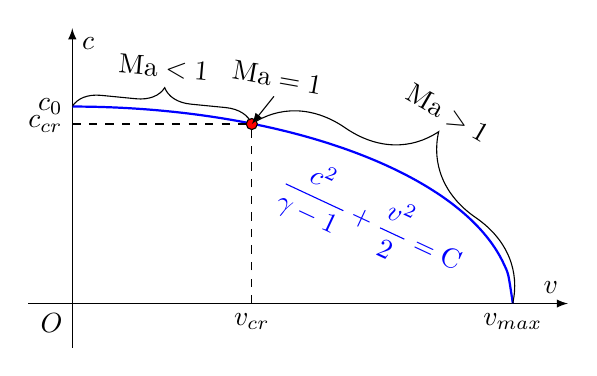
\begin{tikzpicture}
      \begin{axis}[
        axis equal image,
        axis lines=middle,
        axis line style={-latex},
        xmin = -0.4, xmax = 4.5,
        ymin = -0.4, ymax = 2.5,
        xtick=\empty,
        ytick=\empty,
        xlabel={$v$},
        ylabel={$c$},
        %title={$c$-$v$曲线平面图},
        ]
        \addplot[smooth, samples=100,domain=0:4, thick, blue] {(3.2-0.2*x^2)^(0.5)};
        \draw[dashed] (axis cs:1.63,0) node[anchor=north]{$v_{cr}$} -- (axis cs:1.63,1.63)
          node(cr)[xshift=8pt,yshift=10pt,rotate=-10,anchor=south]{$\mathrm{Ma}=1$};
        \draw[dashed] (axis cs:0,1.63) node[anchor=east]{$c_{cr}$} -- (axis cs:1.63,1.63);
        \draw (axis cs:0,1.79) node[anchor=east]{$c_{0}$};
        \node at (axis cs:4,0) [anchor=north]{$v_{max}$};
        \node at (axis cs:0,0) [anchor=north east] {$O$};
        \draw[decorate,decoration={brace, amplitude=10pt}] (axis cs:0,1.79)
          --node[midway, yshift=10pt,rotate=-5,anchor=south]{$\mathrm{Ma}<1$}
          (axis cs:1.63,1.63);
        \draw[decorate,decoration={brace, amplitude=36pt}] (axis cs:1.63,1.63)
          --node[midway, xshift=20pt,yshift=30pt,rotate=-30,anchor=south]{$\mathrm{Ma}>1$}
          (axis cs:4,0);
        \draw[fill=red] (axis cs:1.63,1.63) circle (2pt);
        \draw[-latex] (cr.south) -- (axis cs:1.63,1.63);
        \draw[blue] (axis cs:2,1.5) node[rotate=-25,anchor=north west] {$\displaystyle \frac{c^{2}}{\gamma-1}+\frac{v^{2}}{2}=\mathrm{C}$};
      \end{axis}
    \end{tikzpicture}
  \end{center}
  \begin{definition}[临界状态]
    一维定常等熵气流的某一截面上的速度等于当地声速时的状态称为临界状态。用下标
    $cr$表示。临界状态下的气流参数称为临界参数,该截面为临界截面。
  \end{definition}
\end{frame}

\begin{frame}{临界状态——续}
 临界状态下:
 \begin{equation*}
   v_{cr}
   =
   c_{cr}
 \end{equation*}
 \begin{equation*}
   \frac{c_{cr}^{2}}{\gamma-1}
   +
   \frac{v_{cr}^{2}}{2}
   =
   \frac{c_{0}^{2}}{\gamma-1}
   =
   \frac{v_{max}^{2}}{2}
 \end{equation*}
 \begin{equation*}
   c_{cr}
   =
   \sqrt{\gamma RT_{cr}}
   =
   \sqrt{\frac{2}{\gamma+1}}c_{0}
   =
   \sqrt{\frac{2\gamma R}{\gamma+1}T_{0}}
   =
   \sqrt{\frac{\gamma-1}{\gamma+1}}v_{max}
 \end{equation*}
 \vspace*{-1em}
 \only<2->{
 \begin{block}{讨论}
   \begin{itemize}
     \item<2-|alert@2> 对于给定气流运动,$c_{cr}$只取决于$T_{0}$
     \item<3-|alert@3> 在绝热流动中,$T_{0}$为常数,$c_{cr}$也是常数
     \item<4-|alert@4> 当地声速$c$是气体所处状态下实际存在的声速;临界声速$c_{cr}$是与气流所处状态相对应的临界状态下的声速
     \item<5-|alert@5> 当$\mathrm{Ma}=1$时,当地声速就是临界声速
   \end{itemize}
 \end{block}
 }
\end{frame}

\subsection{一维定常等熵气流中各参数关系式}
\subsubsection{以马赫数$\mathrm{Ma}$为变量的各参数关系式}
\begin{frame}{以马赫数$\mathrm{Ma}$为变量的各参数关系式}
  \vspace*{-1em}
  \begin{equation*}
    h
    +
    \frac{v^{2}}{2}
    =
    h_{0}
    \quad\quad
    c_{p}T
    +
    \frac{v^{2}}{2}
    =
    c_{p}T_{0}
    \quad\quad
    \frac{c^{2}}{\gamma-1}
    +
    \frac{v^{2}}{2}
    =
    \frac{c_{0}^{2}}{\gamma-1}
  \end{equation*}
  %\begin{equation*}
    %h
    %=
    %c_{p}T
  %\end{equation*}
  %\begin{equation*}
    %c_{p}
    %=
    %\frac{\gamma}{\gamma-1}R
  %\end{equation*}
  %\begin{equation*}
  %c
  %=
  %\sqrt{\gamma RT}
  %\end{equation*}
  %\begin{equation*}
    %\mathrm{Ma}
    %=
    %\frac{v}{c}
  %\end{equation*}
  \begin{equation*}
    \frac{T_{0}}{T}
    =
    \frac{c_{0}^{2}}{c^{2}}
    =
    1
    +
    \frac{\gamma-1}{2}\mathrm{Ma}^{2}
  \end{equation*}
  由等熵过程关系式:
  \begin{equation*}
    \frac{p}{\rho^{\gamma}}
    =
    \mathrm{C}
    \quad
    \rightarrow
    \quad
    \frac{p_{0}}{p}
    =
    \left(\frac{\rho_{0}}{\rho}\right)^{\gamma}
    =
    \left(\frac{T_{0}}{T}\right)^{\frac{\gamma}{\gamma-1}}
  \end{equation*}
  \begin{equation*}
    \frac{p_{0}}{p}
    =
    \left(1+\frac{\gamma-1}{2}\mathrm{Ma}^{2}\right)^{\frac{\gamma}{\gamma-1}}
  \end{equation*}
  \begin{equation*}
    \frac{\rho_{0}}{\rho}
    =
    \left(1+\frac{\gamma-1}{2}\mathrm{Ma}^{2}\right)^{\frac{1}{\gamma-1}}
  \end{equation*}
\end{frame}

\subsubsection{以速度系数$M_{*}$为变量的各参数关系式}
\begin{frame}{以速度系数$M_{*}$为变量的各参数关系式}
  \begin{itemize}
    \item 速度系数$M_{*}$表示气流速度与临界声速之比
      \begin{equation*}
        M_{*}
        =
        \frac{v}{c_{cr}}
      \end{equation*}
  \end{itemize}
  \vspace*{-1.5em}
  \begin{columns}[c]
    \begin{column}{0.45\textwidth}
  \begin{equation*}
    \frac{c^{2}}{\gamma-1}
    +
    \frac{v^{2}}{2}
    =
    \frac{c_{cr}^{2}}{\gamma-1}
    +
    \frac{c_{cr}^{2}}{2}
  \end{equation*}
  \begin{equation*}
    \frac{1}{\gamma-1}\frac{1}{\mathrm{Ma}^{2}}
    +
    \frac{1}{2}
    =
    \frac{\gamma+1}{2(\gamma-1)}\frac{1}{M_{*}^{2}}
  \end{equation*}
  \begin{equation*}
    M_{*}^{2}
    =
    \frac{(\gamma+1)\mathrm{Ma}^{2}}{2+(\gamma-1)\mathrm{Ma}^{2}}
  \end{equation*}
  \begin{equation*}
    \mathrm{Ma}^{2}
    =
  \frac{2M_{*}^{2}}{(\gamma+1)+(\gamma-1)M_{*}^{2}}
  \end{equation*}
    \end{column}
  
    \begin{column}{0.55\textwidth}
      \begin{center}
        \adjustbox{width=7cm}{
          % To Do
      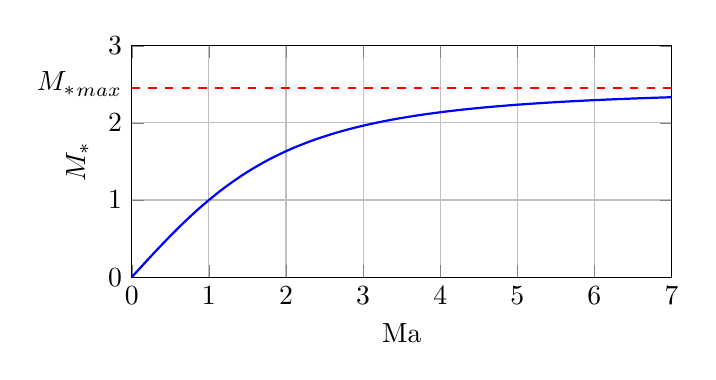
\begin{tikzpicture}
        \begin{axis}[
          axis equal image,
          xmin = 0, xmax = 7,
          ymin = 0, ymax = 3,
          xlabel={$\mathrm{Ma}$},
          ylabel={$M_{*}$},
          grid,
          ]
          \addplot[domain=0:7,smooth,thick,blue]{sqrt((2.4*x^2)/(2+0.4*x^2))};
          \addplot[domain=0:7,dashed,thick,red]{sqrt(6)};
        \end{axis}
          \node at (0,2.45) [anchor=east] {${M_{*}}_{max}$};
      \end{tikzpicture}
    }
      \end{center}
    \end{column}
  \end{columns}
\end{frame}

\begin{frame}{$M_{*}$表示的各参数关系式——续}
  \vspace*{-1.5em}
 \begin{equation*}
   \frac{T}{T_{0}}
   =
   \frac{c^{2}}{c_{0}^{2}}
   =
   1
   -
   \frac{\gamma-1}{\gamma+1}M_{*}^{2}
 \end{equation*} 
 \begin{equation*}
   \frac{p}{p_{0}}
   =
   \left(1-\frac{\gamma-1}{\gamma+1}M_{*}^{2}\right)^{\frac{\gamma}{\gamma-1}}
 \end{equation*}
 \begin{equation*}
   \frac{\rho}{\rho_{0}}
   =
   \left(1-\frac{\gamma-1}{\gamma+1}M_{*}^{2}\right)^{\frac{1}{\gamma-1}}
 \end{equation*}
  \vspace*{-1.5em}
 \begin{block}{讨论}
   \begin{enumerate}
     \item 使用$M_{*}$计算气流速度$v$比使用$\mathrm{Ma}$方便
     \item 在极限状态下,$\mathrm{Ma}=\infty$,
     $M_{*}=v_{max}/c_{cr}=\sqrt{(\gamma+1)/(\gamma-1)}$
     \item $M_{*}$也可作为流动类型的判别标准
       \begin{itemize}
         \item $\mathrm{Ma}<1$,$M_{*}<1$,亚声速流
         \item $\mathrm{Ma}=1$,$M_{*}=1$,声速流
         \item $\mathrm{Ma}>1$,$M_{*}>1$,超声速流
       \end{itemize}
   \end{enumerate}
 \end{block}
\end{frame}

\begin{frame}{临界参数与滞止参数的关系式}
  \vspace*{-1.5em}
  \begin{equation*}
    \left\{
      \begin{aligned}
    \frac{T_{0}}{T}
    &=
    1+\frac{\gamma-1}{2}\mathrm{Ma}^{2}
    \\
    \frac{p_{0}}{p}
    &=
    \left(1+\frac{\gamma-1}{2}\mathrm{Ma}^{2}\right)^{\frac{\gamma}{\gamma-1}}
    \\
    \frac{\rho_{0}}{\rho}
    &=
    \left(1+\frac{\gamma-1}{2}\mathrm{Ma}^{2}\right)^{\frac{1}{\gamma-1}}
      \end{aligned}
    \right.
    \xrightarrow{
      \mathrm{Ma}=1
  }
    \left\{
    \begin{aligned}
    \frac{T_{cr}}{T_{0}}
    &=
    \frac{c_{cr}^{2}}{c_{0}^{2}}
    =
    \frac{2}{\gamma+1}
    \\
    \frac{p_{cr}}{p_{0}}
    &=
    \left(\frac{2}{\gamma+1}\right)^{\frac{\gamma}{\gamma-1}}
    \\
    \frac{\rho_{cr}}{\rho_{0}}
    &=
    \left(\frac{2}{\gamma+1}\right)^{\frac{1}{\gamma-1}}
    \end{aligned}
    \right.
  \end{equation*}
  \vspace*{-1.5em}
  \begin{block}{讨论}
    \begin{itemize}
      %\item 临界参数与滞止参数的比值时常数
      \item 若$\gamma=1.4$,$\displaystyle \frac{T_{cr}}{T_{0}}=0.8333$,
        $\displaystyle \frac{p_{cr}}{p_{0}}=0.5283$,$\displaystyle
        \frac{\rho_{cr}}{\rho_{0}}=0.6339$,声速流动
      \item 若$\displaystyle \frac{T}{T_{0}}>0.8333$,
        $\displaystyle \frac{p}{p_{0}}>0.5283$,$\displaystyle
        \frac{\rho}{\rho_{0}}>0.6339$,亚声速流动
      \item 若$\displaystyle \frac{T}{T_{0}}<0.8333$,
        $\displaystyle \frac{p}{p_{0}}<0.5283$,$\displaystyle
        \frac{\rho}{\rho_{0}}<0.6339$,超声速流动
    \end{itemize}
  \end{block}
\end{frame}

\begin{frame}{各参数关系式示例}
  \vspace*{-0.5em}
  \begin{block}{例:气体在一无摩擦的渐缩管道中流动,已知截面1的压强为
      $p_{1}=2.67\times10^{5}\mathrm{Pa}$,温度为$T_{1}=330\mathrm{K}$,流速为
      $v_{1}=157\mathrm{m/s}$,并且在管道出口截面2达到临界状态。试求气流在出口截
      面的压强、密度、温度和速度。假定气体为空气,$\gamma=1.4$,
      $R=287\mathrm{J/(kg\cdot K)}$。
   }
   \only<2>{解: 首先计算截面1的声速$c_{1}$,马赫数$\mathrm{Ma}_{1}$,滞止压强$p_{0}$和滞
   止温度$T_{0}$
   \vspace{-0.5em}
   \begin{equation*}
     c_{1}
     =
     \sqrt{\gamma RT_{1}}
     =
     \sqrt{1.4\times287\times330}
     =
     364.1\mathrm{m/s}
   \end{equation*}
   \begin{equation*}
     \mathrm{Ma}_{1}
     =
     \frac{v_{1}}{c_{1}}
     =
     \frac{157}{364.1}
     =
     0.4312
   \end{equation*}
   \begin{equation*}
     \frac{T_{0}}{T_{1}}
     =
     1+\frac{\gamma-1}{2}\mathrm{Ma}_{1}^{2}
     =
     1 + \frac{1.4-1}{2}\times0.4312^{2}
     =
     1.037
   \end{equation*}
   \begin{equation*}
     T_{0}
     =
     T_{1}
     \left(1+\frac{\gamma-1}{2}\mathrm{Ma}_{1}^{2}\right)
     =
     330\times1.037
     =
     342.3\mathrm{K}
   \end{equation*}
 }
 \only<3>{
   \begin{equation*}
   \frac{\gamma}{\gamma-1}
   =
   \frac{1.4}{1.4-1}
   =
   3.5
   \end{equation*}
   \begin{equation*}
     p_{0}
     =
     p_{1}
     \left(1+\frac{\gamma-1}{2}\mathrm{Ma}_{1}^{2}\right)^{\frac{\gamma}{\gamma-1}}
     =
     2.67\times10^{5}\times1.037^{3.5}
     =
     3.034\times10^{5}\mathrm{Pa}
   \end{equation*}
   \begin{equation*}
   \frac{2}{\gamma+1}
   =
   \frac{2}{1.4+1}
   =
   0.833
   \end{equation*}
   \begin{equation*}
     p_{2}
     =
     p_{cr}
     =
     p_{0}\left(\frac{2}{\gamma+1}\right)^{\frac{\gamma}{\gamma-1}}
     =
     3.034\times10^{5}\times0.833^{3.5}
     =
     1.411\times10^{5}\mathrm{Pa}
   \end{equation*}
 }
 \only<4>{
   \begin{equation*}
     T_{2}
     =
     T_{cr}
     =
     T_{0}\frac{2}{\gamma+1}
     =
     342.3\times0.833
     =
     285.25\mathrm{K}
   \end{equation*}
   \begin{equation*}
     \rho_{2}
     =
     \rho_{cr}
     =
     \frac{p_{cr}}{RT_{cr}}
     =
     \frac{1.411\times10^{5}}{287\times285.25}
     =
     1.724\mathrm{kg/m^{3}}
   \end{equation*}
   \begin{equation*}
     v_{2}
     =
     c_{cr}
     =
     \sqrt{\gamma RT_{cr}}
     =
     \sqrt{1.4\times287\times285.25}
     =
     338.5\mathrm{m/s}
   \end{equation*}
 }
 \end{block} 
\end{frame}


\section{正激波}
%\section{正激波}
\begin{frame}{激波}
  \begin{columns}[c]
    \begin{column}{0.6\textwidth}
      \begin{itemize}[<+-|alert@+>]
        \item 在气流通过强压缩波时,气流受到突然的压缩,其压强、温度和密度等都将
          突跃地升高,而速度则突跃地降低。这种突跃变化的强压缩波称为
          {\color{blue}激波}
        \item 按照激波的形状,可将激波划分为:
      \end{itemize}
      \only<3>{
        \begin{enumerate}
          \item {\color{blue}正激波}。波面与气流方向相垂直的平面激波,气流通过薄面后,不改变流动方向
            \begin{center}
              \begin{tikzpicture}
                \draw[thick,red] (1, -1) -- (1, 1);
                \draw[-latex] (0,0) -- node[midway, above,anchor=south west]{$v_{1}$} (0.5,0);
                \draw[-latex] (1.5,0) -- node[midway, above,anchor=south west]{$v_{2}$} (2.0,0);
              \end{tikzpicture}
            \end{center}
        \end{enumerate}
      }
      \only<4>{
        \begin{enumerate}
          \setcounter{enumi}{1}
        \item {\color{blue}斜激波}。波面与气流方向不垂直的平面激波,气流通过波面后,要改变流动方向
          \begin{center}
            \begin{tikzpicture}
              \def\firstcircle{(1,0) circle (1.3cm)}
              \draw[thick,red] (1,0) -- ++(30:1.5);
              \draw[thick,red] (1,0) -- ++(-30:1.5);
              \begin{scope}
                \clip \firstcircle;
              \filldraw[thick,pattern=north east lines] (1, 0) -- (2.5, 0.4) -- (2.5, -0.4) -- cycle;
            \end{scope}
            \draw[-latex] (0,0) -- (0.5,0);
          \end{tikzpicture}
        \end{center}
    \end{enumerate}
  }
  \only<5>{
    \begin{enumerate}
      \setcounter{enumi}{2}
    \item {\color{blue}脱体激波}。波形是弯曲的,也称为曲激波。当超声速气流流过钝头物体时,物体的前面将产生脱体激波
      \begin{center}
        \begin{tikzpicture}
          \draw[-latex] (0,0) -- (0.5,0);
          \begin{scope}
            \clip (0.8,-1.3) rectangle (1.2, 1.3);
          \draw[thick, red] (5,0) circle (4cm);
        \end{scope}
        \begin{scope}
          \clip (1.5,0) circle (0.6);
        \filldraw[thick,pattern=north east lines] (2,0) ellipse (0.5cm and 0.3cm);
      \end{scope}
    \end{tikzpicture}
  \end{center}
          \end{enumerate}
        }
      \end{column}
      \begin{column}{0.4\textwidth}
        \begin{figure}
          \includegraphics[width=5cm]{img/shockwave.jpg}
        \end{figure}
      \end{column}
    \end{columns}
  \end{frame}

\subsection{激波的形成}
\begin{frame}{激波的形成}
  \begin{columns}[c]
    \begin{column}{0.4\textwidth}
  \vspace*{-1em}
  \begin{center}
  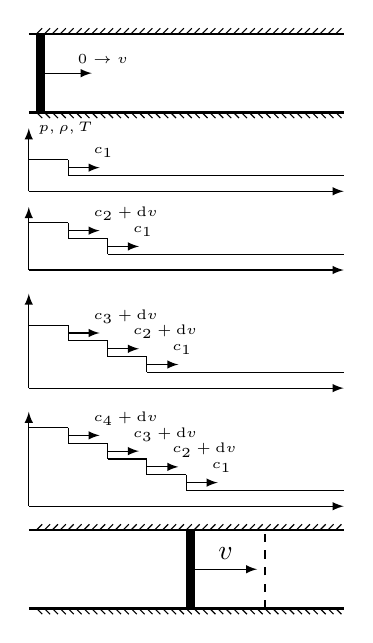
\begin{tikzpicture}
    \begin{scope}
      \draw[thick] (0,0) -- (4,0);
      \draw[thick] (0,1) -- (4,1);
      \draw[fill=black] (0.1,0) rectangle (0.2,1);
    \foreach \p in 
    {0.1, 0.2, 0.3, 0.4, 0.5, 0.6, 0.7, 0.8, 0.9, 1.0,
     1.1, 1.2, 1.3, 1.4, 1.5, 1.6, 1.7, 1.8, 1.9, 2.0,
     2.1, 2.2, 2.3, 2.4, 2.5, 2.6, 2.7, 2.8, 2.9, 3.0,
     3.1, 3.2, 3.3, 3.4, 3.5, 3.6, 3.7, 3.8, 3.9}
    {
      \draw[thin] (\p, 0) -- ++(-45:0.1);
      \draw[thin] (\p, 1) -- ++(45:0.1);
    }
    \draw[-latex] (0.2,0.5) -- node[pos=0.5,above,anchor=south west]{\tiny $0\rightarrow v$} (0.8,0.5);
    \end{scope}
    \begin{scope}[yshift=-1.0cm]
      \draw[-latex](0,0) -- (4,0);
      \draw[-latex](0,0) -- (0,0.8) node[right]{\tiny $p,\rho, T$};
      \draw (0,0.4) -- (0.5,0.4);
      \draw (0.5,0.4) -- (0.5,0.2);
      \draw[-latex] (0.5,0.3) -- node[midway,anchor=south west]{\tiny $c_{1}$}(0.9,0.3);
      \draw (0.5,0.2) -- (4,0.2);
    \end{scope}
    \begin{scope}[yshift=-2.0cm]
      \draw[-latex](0,0) -- (4,0);
      \draw[-latex](0,0) -- (0,0.8);
      \draw (0,0.6) -- (0.5,0.6);
      \draw (0.5,0.6) -- (0.5,0.4);
      \draw[-latex] (0.5,0.5) -- node[midway,anchor=south west]{\tiny $c_{2}+\mathrm{d}v$}(0.9,0.5);
      \draw (0.5,0.4) -- (1,0.4);
      \draw (1,0.4) -- (1,0.2);
      \draw[-latex] (1,0.3) -- node[midway,anchor=south west]{\tiny $c_{1}$}(1.4,0.3);
      \draw (1,0.2) -- (4,0.2);
    \end{scope}
    \begin{scope}[yshift=-3.5cm]
      \draw[-latex](0,0) -- (4,0);
      \draw[-latex](0,0) -- (0,1.2);
      \draw (0,0.8) -- (0.5,0.8);
      \draw (0.5,0.8) -- (0.5,0.6);
      \draw[-latex] (0.5,0.7) -- node[midway,anchor=south west]{\tiny $c_{3}+\mathrm{d}v$}(0.9,0.7);
      \draw (0.5,0.6) -- (1,0.6);
      \draw (1.0,0.6) -- (1,0.4);
      \draw[-latex] (1.0,0.5) -- node[midway,anchor=south west]{\tiny $c_{2}+\mathrm{d}v$}(1.4,0.5);
      \draw (1,0.4) -- (1.5,0.4);
      \draw (1.5,0.4) -- (1.5,0.2);
      \draw[-latex] (1.5,0.3) -- node[midway,anchor=south west]{\tiny $c_{1}$}(1.9,0.3);
      \draw (1.5,0.2) -- (4,0.2);
    \end{scope}
    \begin{scope}[yshift=-5.0cm]
      \draw[-latex](0,0) -- (4,0);
      \draw[-latex](0,0) -- (0,1.2);
      \draw (0,1) -- (0.5,1);
      \draw (0.5,1) -- (0.5,0.8);
      \draw[-latex] (0.5,0.9) -- node[midway,anchor=south west]{\tiny $c_{4}+\mathrm{d}v$}(0.9,0.9);
      \draw (0.5,0.8) -- (1,0.8);
      \draw (1,0.8) -- (1,0.6);
      \draw[-latex] (1,0.7) -- node[midway,anchor=south west]{\tiny $c_{3}+\mathrm{d}v$}(1.4,0.7);
      \draw (1,0.6) -- (1.5,0.6);
      \draw (1.5,0.6) -- (1.5,0.4);
      \draw[-latex] (1.5,0.5) -- node[midway,anchor=south west]{\tiny $c_{2}+\mathrm{d}v$}(1.9,0.5);
      \draw (1.5,0.4) -- (2,0.4);
      \draw (2.0,0.4) -- (2,0.2);
      \draw[-latex] (2,0.3) -- node[midway,anchor=south west]{\tiny$c_{1}$}(2.4,0.3);
      \draw (2.0,0.2) -- (4,0.2);
    \end{scope}
    \begin{scope}[yshift=-6.3cm]
      \draw[thick] (0,0) -- (4,0);
      \draw[thick] (0,1) -- (4,1);
      \draw[fill=black] (2,0) rectangle (2.1,1);
    \foreach \p in 
    {0.1, 0.2, 0.3, 0.4, 0.5, 0.6, 0.7, 0.8, 0.9, 1.0,
     1.1, 1.2, 1.3, 1.4, 1.5, 1.6, 1.7, 1.8, 1.9, 2.0,
     2.1, 2.2, 2.3, 2.4, 2.5, 2.6, 2.7, 2.8, 2.9, 3.0,
     3.1, 3.2, 3.3, 3.4, 3.5, 3.6, 3.7, 3.8, 3.9}
    {
      \draw[thin] (\p, 0) -- ++(-45:0.1);
      \draw[thin] (\p, 1) -- ++(45:0.1);
    }
    \draw[-latex] (2.1,0.5) -- node[midway,above]{$v$} (2.9,0.5);
    \draw[dashed] (3,0) -- (3,1);
    \end{scope}
  \end{tikzpicture}
  \end{center}
    \end{column}
  
    \begin{column}{0.6\textwidth}
    \only<2-4>{
\begin{itemize}[<+(1)->]
  \item 现有一个充满静止气体的长直圆管,管中有一活塞。该活塞向右作突然加速运动,其速度从零加速到某一速度$v$,之后以该速度作匀速运动。
  \item 把这个扰动过程分成无数个微小的阶段。每个微小阶段均是一个微弱压缩扰动。设
    每个微弱压缩扰动产生微小压强增量$\mathrm{d}p$,每个微小阶段活塞速度增加
    $\mathrm{d}v$
  \item 当活塞开始运动时,产生的第一个微弱扰动波以声速$c_{1}$传播,扰动后气体获得与活塞相同的速度$\mathrm{d}v$,压强为
    $p_{2}=p_{1}+\mathrm{d}p$,密度为$\rho_{2}=\rho_{1}+\mathrm{d}\rho$,温度为
    $T_{2}=T_{1}+\mathrm{d}T$
\end{itemize}
}
\only<5-7>{
  \begin{itemize}[<+(4)->]
  \item 紧接着产生第二个微弱扰动波,并在被第一个微弱扰动波扰动过的气体中传播。第
    二个微弱扰动波的声速$c_{2}=\sqrt{\gamma RT_{2}}$,波速为$c_{2}+\mathrm{d}v$
    。扰动后活塞速度又增加$\mathrm{d}v$,气体速度为$2\mathrm{d}v$,压强为
    $p_{3}=p_{2}+\mathrm{d}p$,密度为$\rho_{3}=\rho_{2}+\mathrm{d}\rho$,温度为
    $T_{3}=T_{2}+\mathrm{d}T$
  \item 接着第三个微弱扰动波产生,并在第二个微弱扰动波扰动过的气体中传播,依次类
    推
    \item $p_{1}<p_{2}<p_{3}<\cdots$,$\rho_{1}<\rho_{2}<\rho_{3}<\cdots$,$T_{1}<T_{2}<T_{3}<\cdots$,$c_{1}<c_{2}<c_{3}<\cdots$,$c_{1}<c_{2}+\mathrm{d}v<c_{3}+2\mathrm{d}v<\cdots$
\end{itemize}
}
\only<8-10>{
  \begin{itemize}[<+(7)->]
    \item 在整个活塞压缩过程中,管道内将产生并形成若干道微弱压缩波,每一个波的传播速度不一样,后一个时刻产生的微弱扰动波的传播速度将大于前一时刻产生的微弱扰动波的传播速度
    \item 经过一段时间后,后产生的微弱扰动波将逐渐接近先产生的微弱扰动波,波与波之间的距离逐渐缩小,波形越来越陡
    \item 最后,后面的波赶上前面的破,所有的微弱扰动波聚集在一起,叠加成一个垂直于流动方向的具有压强不连续面的强压缩波,即正激波
  \end{itemize}
}
\only<11->{
  \vspace*{-1em}
  \begin{itemize}[<+(10)->]
    \item 往后,随着活塞匀速$v$继续运动,管道内能维持一个强度不变的正激波
    \item 正激波后面受到扰动的气体,其速度由扰动前的零增加到与活塞相同的速度$v$
    \item 正激波传播速度大于未受扰动气体的声速$c_{1}$
    \item 正激波的这种突跃变化是不连续的,是在与气体分子平面自由程同一数量级内完
      成(空气约$3\times10^{-4}\mathrm{mm}$)
    \item 宏观上可以认为是在一个几何面上突然变化的,即激波是不连续的间断面,气流
      通过激波的变化是突然的、不连续的
  \end{itemize}
}
    \end{column}
    
  \end{columns}
\end{frame}

\subsection{正激波的基本方程}
\begin{frame}{正激波的基本方程}
  \vspace*{-1em}
  \begin{center}
  \begin{tikzpicture}
\begin{scope}
    \draw[thick] (0,0) -- (5,0);
    \draw[thick] (0,1.5) -- (5,1.5);
    %\draw[thick] (2,0) node[anchor=north]{$n$} -- (2,1.5) node[anchor=south]{$m$};
    \filldraw[thick,pattern=north east lines] (2.6,0) -- (2.6,1.5) -- (2.4,1.5)
      -- (2.4, 0) -- cycle;
    \draw[thick,-latex] (2.5,0.75) -- node[midway,above]{$v_{s}$} node[midway,below]{$p_{1}$}(3.5,0.75);
    \draw[thick,-latex] (1.0,0.75) -- node[midway,above]{$v_{g}$}
      node[midway,below]{$p_{2}$} (2.2,0.75);
    \foreach \p in 
    {0.1, 0.2, 0.3, 0.4, 0.5, 0.6, 0.7, 0.8, 0.9, 1.0,
     1.1, 1.2, 1.3, 1.4, 1.5, 1.6, 1.7, 1.8, 1.9, 2.0,
     2.1, 2.2, 2.3, 2.4, 2.5, 2.6, 2.7, 2.8, 2.9, 3.0,
     3.1, 3.2, 3.3, 3.4, 3.5, 3.6, 3.7, 3.8, 3.9, 4.0,
     4.1, 4.2, 4.3, 4.4, 4.5, 4.6, 4.7, 4.8, 4.9}
    {
      \draw[thin] (\p, 0) -- ++(-45:0.1);
      \draw[thin] (\p, 1.5) -- ++(45:0.1);
    }
  \end{scope}
  \begin{scope}[xshift=6cm]
    \draw[thick] (0,0) -- (5,0);
    \draw[thick] (0,1.5) -- (5,1.5);
    %\draw[thick] (2,0) node[anchor=north]{$n$} -- (2,1.5) node[anchor=south]{$m$};
    \filldraw[thick,pattern=north east lines] (2.6,0) -- (2.6,1.5) -- (2.4,1.5)
      -- (2.4, 0) -- cycle;
    \draw[dashed,thick] (2.3,0) node[below,anchor=north]{$2$} -- (2.3,1.5)
      node[above,anchor=south]{$2$};
    \draw[dashed,thick] (2.7,0) node[below,anchor=north]{$1$} -- (2.7,1.5)
      node[above,anchor=south]{$1$};
    \draw[thick,-latex] (2.0,0.75) -- node[midway,above]{$v_{2}=v_{s}-v_{g}$} node[midway,below]{$p_{2}$} (0.2,0.75);
    \draw[thick,-latex] (4.8,0.75) -- node[midway,above]{$v_{1}=v_{s}$} node[midway,below]{$p_{1}$}(3.0,0.75);
    \foreach \p in 
    {0.1, 0.2, 0.3, 0.4, 0.5, 0.6, 0.7, 0.8, 0.9, 1.0,
     1.1, 1.2, 1.3, 1.4, 1.5, 1.6, 1.7, 1.8, 1.9, 2.0,
     2.1, 2.2, 2.3, 2.4, 2.5, 2.6, 2.7, 2.8, 2.9, 3.0,
     3.1, 3.2, 3.3, 3.4, 3.5, 3.6, 3.7, 3.8, 3.9, 4.0,
     4.1, 4.2, 4.3, 4.4, 4.5, 4.6, 4.7, 4.8, 4.9}
    {
      \draw[thin] (\p, 0) -- ++(-45:0.1);
      \draw[thin] (\p, 1.5) -- ++(45:0.1);
    }
  \end{scope}
  \end{tikzpicture}
  \end{center}
  取激波两侧的1-1、2-2两个断面之间气流组成控制体。

  连续性方程:
  \begin{equation*}
    \rho_{1}v_{1}
    =
    \rho_{2}v_{2}
  \end{equation*}
  动量方程:
  \begin{equation*}
    p_{1}-p_{2}
    =
    \rho_{1}v_{1}(v_{2}-v_{1})
  \end{equation*}
  \begin{equation*}
    p_{1}
    +
    \rho_{1}v_{1}^{2}
    =
    p_{2}
    +
    \rho_{2}v_{2}^{2}
  \end{equation*}
  能量方程:
  \begin{equation*}
    h_{1}
    +
    \frac{v_{1}^{2}}{2}
    =
    h_{2}
    +
    \frac{v_{2}^{2}}{2}
  \end{equation*}
\end{frame}

\subsection{兰金-许贡纽公式}
\begin{frame}{兰金-许贡纽公式(Rankine-Hugoniot)}
  \vspace*{-1em}
  \begin{equation*}
    \rho_{1}v_{1}
    =
    \rho_{2}v_{2}
  \end{equation*}
  \begin{equation*}
    p_{1}-p_{2}
    =
    \rho_{1}v_{1}(v_{2}-v_{1})
  \end{equation*}
  \begin{equation*}
  v_{1}-v_{2}
  =
  \frac{p_{2}}{\rho_{2}v_{2}}
  -
  \frac{p_{1}}{\rho_{1}v_{1}}
  \quad\quad\quad
    v_{1}+v_{2}
    =
    \frac{\rho_{1}v_{1}}{\rho_{1}}
    +
    \frac{\rho_{2}v_{2}}{\rho_{2}}
  \end{equation*}
  \begin{equation*}
    \begin{aligned}
    v_{1}^{2}-v_{2}^{2}
    &=
    \left(
  \frac{p_{2}}{\rho_{2}v_{2}}
  -
  \frac{p_{1}}{\rho_{1}v_{1}}
    \right)
    \left(
    \frac{\rho_{1}v_{1}}{\rho_{1}}
    +
    \frac{\rho_{2}v_{2}}{\rho_{2}}
    \right)
    %两个括号内的分母和分子可以相互抵消
    \\
    &=
    (p_{2}-p_{1})
    \left(\frac{1}{\rho_{2}}+\frac{1}{\rho_{1}}\right)
    \end{aligned}
  \end{equation*}
  \begin{equation*}
    h_{1}
    +
    \frac{v_{1}^{2}}{2}
    =
    h_{2}
    +
    \frac{v_{2}^{2}}{2}
  \end{equation*}
  \begin{equation*}
    \tikzmarkin<2->[h2]{c7s5s1t1}
    h_{2}-h_{1}
    =
    \frac{1}{2}\left(\frac{1}{\rho_{2}}+\frac{1}{\rho_{1}}\right)
    (p_{2}-p_{1})
    \tikzmarkend{c7s5s1t1}
  \end{equation*}
    \onslide<2->{
    \begin{tikzpicture}[remember picture, overlay]
      \coordinate (c7s5s1t1-aa) at ($(c7s5s1t1)+(7.2,-0.25)$);
      \node[align=left,above,red] at (c7s5s1t1-aa) {\small 兰金-许贡纽公式};
      \path[-latex,red, draw] (c7s5s1t1-aa) |- ($(c7s5s1t1)+(5.75,-0.5)$);
    \end{tikzpicture}
  }
\end{frame}

\begin{frame}{压强突变与密度突变对应关系}
  \vspace*{-1.5em}
  \begin{equation*}
    h_{2}-h_{1}
    =
    \frac{1}{2}\left(\frac{1}{\rho_{2}}+\frac{1}{\rho_{1}}\right)
    (p_{2}-p_{1})
  \end{equation*}
 对于完全气体
 \vspace*{-1em}
 \begin{equation*}
 h
 =
 \frac{\gamma}{\gamma-1}\frac{p}{\rho}
 \end{equation*}
 \begin{equation*}
   \frac{\gamma}{\gamma-1}\frac{p_{2}}{\rho_{2}}
   -
   \frac{\gamma}{\gamma-1}\frac{p_{1}}{\rho_{1}}
   =
    \frac{1}{2}\left(\frac{1}{\rho_{2}}+\frac{1}{\rho_{1}}\right)
    (p_{2}-p_{1})
 \end{equation*}
 \only<2-5>{
   \begin{equation*}
   \frac{\gamma}{\gamma-1}
   \frac{p_{2}\rho_{1}-p_{1}\rho_{2}}{\rho_{1}\rho_{2}}
   =
   \frac{1}{2}
   \frac{\rho_{1}+\rho_{2}}{\rho_{1}\rho_{2}}(p_{2}-p_{1})
   \end{equation*}
 }
 \only<3-5>{
   \begin{equation*}
   \frac{\gamma}{\gamma-1}
 (p_{2}\rho_{1}-p_{1}\rho_{2})
   =
   \frac{1}{2}
   (\rho_{1}+\rho_{2})(p_{2}-p_{1})
   =
   \frac{1}{2}
   (p_{2}\rho_{1}-p_{1}\rho_{2})
   +
   \frac{1}{2}
   (p_{2}\rho_{2}-p_{1}\rho_{1})
   \end{equation*}
 }
 \only<4-5>{
   \begin{equation*}
     \frac{\gamma+1}{\gamma-1}(p_{2}\rho_{1}-p_{1}\rho_{2})
     =
     (p_{2}\rho_{2}-p_{1}\rho_{1})
   \end{equation*}
 }
 \only<5-6>{
   \begin{equation*}
   \frac{\gamma+1}{\gamma-1}
   \left(\frac{p_{2}}{p_{1}}-\frac{\rho_{2}}{\rho_{1}}\right)
   =
   \frac{p_{2}}{p_{1}}\frac{\rho_{2}}{\rho_{1}}-1
   \end{equation*}
 }
 \only<6>{
   \begin{equation*}
     \left(\frac{\gamma+1}{\gamma-1}-\frac{\rho_{2}}{\rho_{1}}\right)\frac{p_{2}}{p_{1}}
     =
     \frac{\gamma+1}{\gamma-1}\frac{\rho_{2}}{\rho_{1}}-1
   \end{equation*}
   \begin{equation*}
     \left(\frac{\gamma+1}{\gamma-1}+\frac{p_{2}}{p_{1}}\right)\frac{\rho_{2}}{\rho_{1}}
     =
     \frac{\gamma+1}{\gamma-1}\frac{p_{2}}{p_{1}}+1
   \end{equation*}
 }
 \uncover<7->{
 \begin{equation*}
   \frac{\rho_{2}}{\rho_{1}}
   =
   \dfrac
   {\dfrac{\gamma+1}{\gamma-1}\dfrac{p_{2}}{p_{1}}+1}
   {\dfrac{\gamma+1}{\gamma-1}+\dfrac{p_{2}}{p_{1}}}
   \quad
   \mbox{或}
   \quad
   \frac{p_{2}}{p_{1}}
   =
   \dfrac
   {\dfrac{\gamma+1}{\gamma-1}\dfrac{\rho_{2}}{\rho_{1}}-1}
   {\dfrac{\gamma+1}{\gamma-1}-\dfrac{\rho_{2}}{\rho_{1}}}
 \end{equation*}
 }
 \uncover<8->{
 \begin{equation*}
   \frac{T_{2}}{T_{1}}
   =
   \frac{p_{2}}{p_{1}}
   \frac{\rho_{1}}{\rho_{2}}
   =
   \frac{p_{2}}{p_{1}}
   \dfrac
   {\dfrac{\gamma+1}{\gamma-1}+\dfrac{p_{2}}{p_{1}}}
   {\dfrac{\gamma+1}{\gamma-1}\dfrac{p_{2}}{p_{1}}+1}
   =
   \dfrac
   {\dfrac{\gamma+1}{\gamma-1}\dfrac{p_{2}}{p_{1}}+\left(\dfrac{p_{2}}{p_{1}}\right)^{2}}
   {\dfrac{\gamma+1}{\gamma-1}\dfrac{p_{2}}{p_{1}}+1}
 \end{equation*}
 }
\end{frame}

\begin{frame}{压强突变与密度突变对应关系图}
  \begin{columns}[c]
    \begin{column}{0.4\textwidth}
      \vspace*{-1em}
 \begin{equation*}
   \begin{aligned}
   \frac{p_{2}}{p_{1}}
   &=
   \dfrac
   {\dfrac{\gamma+1}{\gamma-1}\dfrac{\rho_{2}}{\rho_{1}}-1}
   {\dfrac{\gamma+1}{\gamma-1}-\dfrac{\rho_{2}}{\rho_{1}}}
   \\
   \frac{T_{2}}{T_{1}}
   &=
   \dfrac
   {\dfrac{\gamma+1}{\gamma-1}\dfrac{p_{2}}{p_{1}}+\left(\dfrac{p_{2}}{p_{1}}\right)^{2}}
   {\dfrac{\gamma+1}{\gamma-1}\dfrac{p_{2}}{p_{1}}+1}
   \end{aligned}
 \end{equation*}
 对于等熵过程:
 \begin{equation*}
   \begin{aligned}
   \frac{p_{2}}{p_{1}}
  & =
   \left(\frac{\rho_{2}}{\rho_{1}}\right)^{\gamma}
   \\
   \frac{T_{2}}{T_{1}}
  & =
   \left(\frac{p_{2}}{p_{1}}\right)^{\frac{\gamma-1}{\gamma}}
   \end{aligned}
 \end{equation*}
    \end{column}
  
    \begin{column}{0.6\textwidth}
      \begin{center}
 \adjustbox{width=\textwidth}
 {
 \begin{tikzpicture}
     \begin{axis}[
       xmin = 0, xmax = 6.5,
       ymin = 0, ymax = 100,
       xlabel = {$\frac{\rho_{2}}{\rho_{1}}$},
       ylabel = {$\frac{p_{2}}{p_{1}}$},
       ylabel style={rotate=-90, anchor=center},
       legend style={
         anchor=south,
         at = {(axis cs:4,72)}},
       ]
     \addplot [domain=0:6.5,thick,smooth,blue]{x^(1.4)};
     \addlegendentry{等熵过程};
     \addplot [domain=0.1667:5.65,thick,smooth,red]{(6*x-1)/(6-x)};
     \addlegendentry{激波过程};
   \end{axis}
 \end{tikzpicture}
 }
      \end{center}
    \end{column}
  \end{columns}
\end{frame}

\begin{frame}[t]{压强突变与密度突变对应关系讨论}
  \vspace*{-0.5em}
  \begin{columns}[c]
   \begin{column}{0.4\textwidth}
     激波过程:
     \begin{equation*}
   \frac{p_{2}}{p_{1}}
   =
   \dfrac
   {\dfrac{\gamma+1}{\gamma-1}\dfrac{\rho_{2}}{\rho_{1}}-1}
   {\dfrac{\gamma+1}{\gamma-1}-\dfrac{\rho_{2}}{\rho_{1}}}
     \end{equation*}
     等熵过程:
     \begin{equation*}
   \frac{p_{2}}{p_{1}}
  =
   \left(\frac{\rho_{2}}{\rho_{1}}\right)^{\gamma}
     \end{equation*}
     \vspace*{1em}
   \end{column}
   \begin{column}{0.6\textwidth}
 \adjustbox{height=6cm}
 {
 \begin{tikzpicture}
     \begin{axis}[
       xmin = 0, xmax = 6.5,
       ymin = 0, ymax = 100,
       xlabel = {$\frac{\rho_{2}}{\rho_{1}}$},
       ylabel = {$\frac{p_{2}}{p_{1}}$},
       ylabel style={rotate=-90, anchor=center},
       legend style={
         anchor=south,
         at = {(axis cs:4,72)}},
       ]
     \addplot [domain=0:6.5,thick,smooth,blue]{x^(1.4)};
     \addlegendentry{等熵过程};
     \only<1-3>{
     \addplot [domain=0.1667:5.65,thick,smooth,red]{(6*x-1)/(6-x)};
     }
     \only<4->{
       \addplot [domain=1:5.65,thick,smooth,red]{(6*x-1)/(6-x)};
     }
     \addlegendentry{激波过程};
     \only<5->{
       \draw[thick,dashed, red] (axis cs:6,0) -- (axis cs:6,100);
       \node[anchor=south,fill=white] at (axis cs:6,20) {$\frac{\gamma+1}{\gamma-1}$};
     }
   \end{axis}
   \only<3-4>{
     \begin{scope}[xshift=0.8cm,yshift=3.4cm]
       \begin{axis}
         [
         tiny,
         axis equal image,
         xmin = 0, xmax = 1,
         ymin = 0, ymax = 1,
         xtick distance = 0.5,
         ytick distance = 0.5,
         ]
         \addplot[domain=0:1,thick,smooth,blue]{x^(1.4)};
         \addplot[domain=0.1667:1,thick,dashed,smooth,red]{(6*x-1)/(6-x)};
       \end{axis}
     \end{scope}
     \begin{scope}[xshift=0.8cm,yshift=0.9cm]
       \begin{axis}
         [
         tiny,
         xmin = 1, xmax = 2.5,
         ymin = 1, ymax = 4,
         xtick distance = 0.5,
         ytick distance = 1,
         ]
         \addplot[domain=1:2.5,thick,smooth,blue]{x^(1.4)};
         \addplot[domain=1:2.5,thick,smooth,red]{(6*x-1)/(6-x)};
       \end{axis}
     \end{scope}
   }
 \end{tikzpicture}
 }
   \end{column}
 \end{columns}
 \vspace*{-0.5em}
 \only<2>{
   \begin{itemize}
     \item 压强比较小时,激波过程与等熵过程几乎重合,即跨过弱激波的过程非常接近于等熵过程
     \item 压强比越大,激波过程与等熵过程差别越大
   \end{itemize}
 }
 \only<3-4>{
   \begin{itemize}
     \item 当$\rho_{2}/\rho_{1}=1$,激波过程与等熵过程相交,$p_{2}/p_{1}=1$
     \item 当$\rho_{2}/\rho_{1}<1$,激波过程低于等熵过程,膨胀波,熵减过程,不存在%违反热力学第二定律,
     \item 当$\rho_{2}/\rho_{1}>1$,激波过程高于等熵过程,压缩波,熵增过程
   \end{itemize}
 }
 \only<5>{
   \begin{itemize}
     \item 在激波过程中,当$p_{2}/p_{1}\rightarrow\infty$,$\rho_{2}/\rho_{1}\rightarrow (\gamma+1)/(\gamma-1)$
     \item 在等熵过程中,当$p_{2}/p_{1}\rightarrow\infty$,$\rho_{2}/\rho_{1}\rightarrow\infty$
   \end{itemize}
 }
\end{frame}

\begin{frame}{压强突变与温度突变对应关系}
  \vspace*{-2em}
  \begin{columns}[c]
    \begin{column}{0.4\textwidth}
  激波过程:
  \begin{equation*}
   \frac{T_{2}}{T_{1}}
   =
   \dfrac
   {\dfrac{\gamma+1}{\gamma-1}\dfrac{p_{2}}{p_{1}}+\left(\dfrac{p_{2}}{p_{1}}\right)^{2}}
   {\dfrac{\gamma+1}{\gamma-1}\dfrac{p_{2}}{p_{1}}+1}
  \end{equation*}
  等熵过程:
  \begin{equation*}
   \frac{T_{2}}{T_{1}}
  =
   \left(\frac{p_{2}}{p_{1}}\right)^{\frac{\gamma-1}{\gamma}}
  \end{equation*}
    \end{column}
  
    \begin{column}{0.6\textwidth}
      \begin{center}
        \adjustbox{width=\textwidth}{
      \begin{tikzpicture}
       \begin{axis}
         [
         xmin = 1, xmax = 3,
         ymin = 1, ymax = 9,
         xtick distance = 1,
         ytick distance = 2,
       xlabel = {$\frac{T_{2}}{T_{1}}$},
       ylabel = {$\frac{p_{2}}{p_{1}}$},
       ylabel style={rotate=-90, anchor=center},
       legend style={
         anchor=south,
         at = {(axis cs:2.5,2.5)}},
         ]
         \addplot[domain=1:2,thick,smooth,blue]{x^(3.5)};
     \addlegendentry{等熵过程};
     \addplot[domain=1:2.6,thick,smooth,red]{3*x-3+((3*x-3)^2+x)^0.5};
     \addlegendentry{激波过程};
       \end{axis}
      \end{tikzpicture}
    }
      \end{center}
    \end{column}
    
  \end{columns}
  \begin{itemize}
    \item 同一压缩比下,激波过程的温度变化大于等于等熵过程的温度变化
  \end{itemize}
\end{frame}


\subsection{正激波前后气流参数的关系}
\begin{frame}{普朗特公式}
  \uncover<1->{
  连续性方程:
  \begin{equation*}
    \rho_{1}v_{1}
    =
    \rho_{2}v_{2}
  \end{equation*}
  动量方程:
  \begin{equation*}
    p_{1}-p_{2}
    =
    \rho_{1}v_{1}(v_{2}-v_{1})
  \end{equation*}
  \begin{equation*}
    v_{1} - v_{2}
    =
    \frac{p_{2}}{\rho_{2}v_{2}} 
    -
    \frac{p_{1}}{\rho_{1}v_{1}} 
  \end{equation*}
}
\uncover<2->{
  考虑声速公式
  \begin{equation*}
    c = \sqrt{\gamma\frac{p}{\rho}}
  \end{equation*}
}
\uncover<3->{
  \begin{equation*}
    v_{1} - v_{2}
    =
    \frac{c_{2}^{2}}{\gamma v_{2}}
    -
    \frac{c_{1}^{2}}{\gamma v_{1}}
  \end{equation*}
}
\uncover<4->{
  能量方程:
  \begin{equation*}
    \frac{c_{1}^{2}}{\gamma-1}
    +
    \frac{v_{1}^{2}}{2}
    =
    \frac{c_{2}^{2}}{\gamma-1}
    +
    \frac{v_{2}^{2}}{2}
    =
    \frac{c_{0}^{2}}{\gamma-1}
    =
    \frac{\gamma+1}{\gamma-1}
    \frac{c_{cr}^{2}}{2}
  \end{equation*}
}
\end{frame}

\begin{frame}{普朗特公式——续1}
  \vspace*{-1.5em}
  \begin{equation*}
    \frac{c_{1}^{2}}{\gamma-1}
    +
    \frac{v_{1}^{2}}{2}
    =
    \frac{c_{2}^{2}}{\gamma-1}
    +
    \frac{v_{2}^{2}}{2}
    =
    \frac{c_{0}^{2}}{\gamma-1}
    =
    \frac{\gamma+1}{\gamma-1}
    \frac{c_{cr}^{2}}{2}
  \end{equation*}
  \only<2-7>{
  \begin{equation*}
    c_{1}^{2}
    =
    \frac{\gamma+1}{2}c_{cr}^{2}
    -
    \frac{\gamma-1}{2}v_{1}^{2}
    \quad\quad
    c_{2}^{2}
    =
    \frac{\gamma+1}{2}c_{cr}^{2}
    -
    \frac{\gamma-1}{2}v_{2}^{2}
  \end{equation*}
}
\vspace*{-0.5em}
\uncover<3->{
  \begin{equation*}
    v_{1} - v_{2}
    =
    \frac{c_{2}^{2}}{\gamma v_{2}}
    -
    \frac{c_{1}^{2}}{\gamma v_{1}}
  \end{equation*}
}
%\vspace*{-0.5em}
\only<4-7>{
  \begin{equation*}
    v_{1}-v_{2}
    =
    \frac{\gamma+1}{2\gamma v_{2}}c_{cr}^{2}
    -
    \frac{\gamma-1}{2\gamma v_{2}}v_{2}^{2}
    -
    \frac{\gamma+1}{2\gamma v_{1}}c_{cr}^{2}
    +
    \frac{\gamma-1}{2\gamma v_{1}}v_{1}^{2}
  \end{equation*}
}
\only<5-7>{
  \begin{equation*}
    \frac{\gamma+1}{2\gamma}v_{1}
    -
    \frac{\gamma+1}{2\gamma}v_{2}
    =
    \frac{\gamma+1}{2\gamma}\frac{v_{1}-v_{2}}{v_{1}v_{2}}c_{cr}^{2}
  \end{equation*}
}
\only<6-7>{
  \begin{equation*}
    \frac{\gamma+1}{\gamma}(v_{1}-v_{2})\left(1-\frac{c_{cr}^{2}}{v_{1}v_{2}}\right)=0
  \end{equation*}
}
\uncover<7->{
  \begin{equation*}
    v_{1}v_{2}=c_{cr}^{2}
  \end{equation*}
}
\vspace*{-1em}
\uncover<8->{
  \begin{equation*}
    \tikzmarkin<9->[h3]{c7s5s1t2}
    {M_{*}}_{1}
    {M_{*}}_{2}
    =
    1
    \tikzmarkend{c7s5s1t2}
  \end{equation*}
}
    \onslide<9->{
    \begin{tikzpicture}[remember picture, overlay]
      \coordinate (c7s5s1t2-aa) at ($(c7s5s1t2)+(4,-0.55)$);
      \node[align=left,above,red] (a) at (c7s5s1t2-aa) {\small 普朗特公式};
      \path[-latex,red, draw] (a.west) -- ($(c7s5s1t2)+(2.25,-0.25)$);
    \end{tikzpicture}
  }
  \uncover<10->{
动量方程:
  \vspace*{-1em}
  \begin{equation*}
    p_{2}-p_{1}
    =
    \rho_{1} v_{1}^{2}
    -
    \rho_{2} v_{2}^{2}
    =
    \rho v_{1}^{2}\left(1-\frac{v_{2}}{v_{1}}\right)
  \end{equation*}
}
\uncover<11->{
  \vspace*{-1em}
  \begin{itemize}
    \item<11-|alert@11> 激波是压缩波,即$p_{2}>p_{1}$,则$v_{2}<v_{1}$
    \item<12-|alert@12> ${M_{*}}_{1}>1$,${M_{*}}_{2}<1$
    \item<13-|alert@13> 波前气流(1断面)为超声速,波后气流(2断面)为亚声速
  \end{itemize}
}
\end{frame}

\begin{frame}{正激波前后马赫数关系}
  \only<1-7>{
  \vspace*{-1.5em}
\begin{equation*}
  {M_{*}}_{1}^{2}
  {M_{*}}_{2}^{2}
  =
  1
\end{equation*}
}
\only<2-7>{
  \vspace*{-1em}
  \begin{equation*}
    M_{*}^{2}
    =
    \frac{(\gamma+1)\mathrm{Ma}^{2}}{2+(\gamma-1)\mathrm{Ma}^{2}}
    \quad\quad
    \mathrm{Ma}^{2}
    =
    \frac{2M_{*}^{2}}{(\gamma+1)-(\gamma-1)M_{*}^{2}}
  \end{equation*}
}
  \only<3-7>{
\begin{equation*}
  \frac{(\gamma+1)\mathrm{Ma}_{1}^{2}}{2+(\gamma-1)\mathrm{Ma}_{1}^{2}}
  \frac{(\gamma+1)\mathrm{Ma}_{2}^{2}}{2+(\gamma-1)\mathrm{Ma}_{2}^{2}}
  =
  1
\end{equation*}
}
  \only<4-7>{
\begin{equation*}
  (\gamma+1)\mathrm{Ma}_{2}^{2}
  =
  \frac{2+(\gamma-1)\mathrm{Ma}_{1}^{2}}{(\gamma+1)\mathrm{Ma}_{1}^{2}}
  \left[2+(\gamma-1)\mathrm{Ma}_{2}^{2}\right]
\end{equation*}
}
  \only<5-7>{
\begin{equation*}
  \left[
(\gamma+1) -
\frac{2+(\gamma-1)\mathrm{Ma}_{1}^{2}}{(\gamma+1)\mathrm{Ma}_{1}^{2}}(\gamma-1)
\right]\mathrm{Ma}_{2}^{2}
=
2
\frac{2+(\gamma-1)\mathrm{Ma}_{1}^{2}}{(\gamma+1)\mathrm{Ma}_{1}^{2}}
\end{equation*}
}
  \only<6-7>{
\begin{equation*}
  \left[
    (\gamma+1)^{2}\mathrm{Ma}_{1}^{2}
    -
    (\gamma-1)^{2}\mathrm{Ma}_{1}^{2}
    -
    2(\gamma-1)
  \right]\mathrm{Ma}_{2}^{2}
  =
2
\left[2+(\gamma-1)\mathrm{Ma}_{1}^{2}\right]
\end{equation*}
}
  \uncover<7->{
\vspace{-0.5em}
\begin{equation*}
  \mathrm{Ma}_{2}^{2}
  =
  \frac{2+(\gamma-1)\mathrm{Ma}_{1}^{2}}{2\gamma \mathrm{Ma}_{1}^{2}-(\gamma-1)}
\end{equation*}
}
\only<8>{
  \begin{center}
    \adjustbox{height=5.5cm}{
  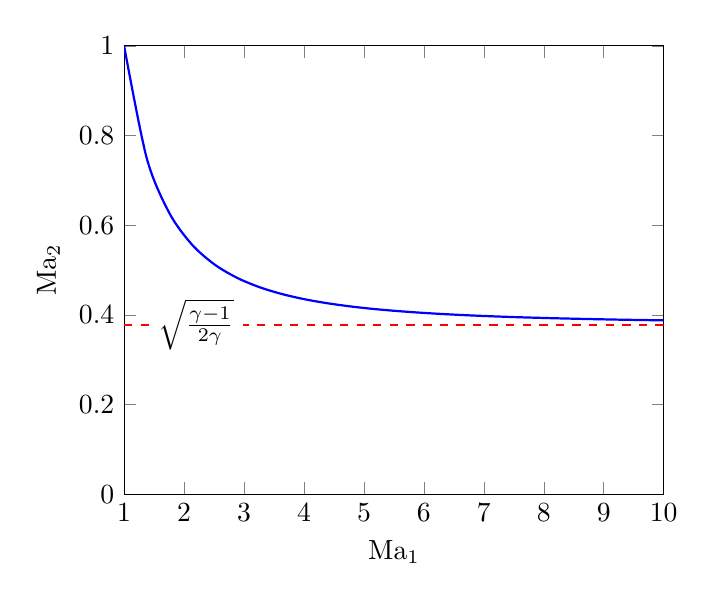
\begin{tikzpicture}
    \begin{axis}[
      xmin=1, xmax=10,
      ymin=0, ymax=1,
      ytick distance = 0.2,
      xtick distance = 1,
      xlabel={$\mathrm{Ma}_{1}$},
      ylabel={$\mathrm{Ma}_{2}$},
      ]
      \addplot[domain=1:10,smooth,thick,blue] {((2+0.4*x^2)/(2.8*x^2-0.4))^0.5};
      \addplot[domain=1:10,smooth,thick,dashed,red] {0.378};
      \node[anchor=center,fill=white] at (2.2,0.378) {$\sqrt{\frac{\gamma-1}{2\gamma}}$};
    \end{axis}
  \end{tikzpicture}
}
  \end{center}
}
\end{frame}

\begin{frame}{$\mathrm{Ma}$或$M_{*}$表示的密度比}
  \begin{itemize}
    \item \color{blue}速度比
  \end{itemize}
 \begin{equation*}
   \frac{v_{1}}{v_{2}}
   =
   \frac{v_{1}^{2}}{v_{1}v_{2}}
   =
   \frac{v_{1}^{2}}{c_{cr}^{2}}
   =
   {M_{*}}_{1}^{2}
   =
   \frac{(\gamma+1)\mathrm{Ma}_{1}^{2}}{2+(\gamma-1)\mathrm{Ma}_{1}^{2}}
 \end{equation*} 
 \uncover<2->{
 连续性方程
 \begin{equation*}
   \rho_{1}v_{1}=\rho_{2}v_{2} 
 \end{equation*}
 }
 \uncover<3->{
  \begin{itemize}
    \item \color{blue}密度比
  \end{itemize}
 \begin{equation*}
   \frac{\rho_{2}}{\rho_{1}}
   =
   \frac{v_{1}}{v_{2}}
   =
   \frac{(\gamma+1)\mathrm{Ma}_{1}^{2}}{2+(\gamma-1)\mathrm{Ma}_{1}^{2}}
 \end{equation*}
 }
\end{frame}

\begin{frame}{$\mathrm{Ma}$或$M_{*}$表示的压强比}
 \uncover<2->{
 动量方程
 \begin{equation*}
   p_{1}-p_{2}
   =
   \rho_{1}v_{2}(v_{2}-v_{1})
 \end{equation*}
 }
 \uncover<3->{
   \vspace*{-0.5em}
 \begin{equation*}
   \frac{p_{2}}{p_{1}}
   \uncover<3->{
     =
   1+\frac{\rho v_{1}}{p_{1}}(v_{1}-v_{2})
 }
 \uncover<4->{
   =
   1+\frac{\gamma v_{1}^{2}}{c_{1}^{2}}\left(1-\frac{v_{2}}{v_{1}}\right)
 }
 \uncover<5->{
   =
   1+\gamma \mathrm{Ma}_{1}^{2}\left(1-\frac{v_{2}}{v_{1}}\right)
 }
 \end{equation*}
 }
 \uncover<6->{
 \begin{equation*}
   \frac{v_{1}}{v_{2}}
   =
   {M_{*}}_{1}^{2}
   =
   \frac{(\gamma+1)\mathrm{Ma}_{1}^{2}}{2+(\gamma-1)\mathrm{Ma}_{1}^{2}}
 \end{equation*} 
 }
 \uncover<7->{
  \begin{itemize}
    \item \color{blue}压强比
  \end{itemize}
 \begin{equation*}
   \begin{aligned}
   \frac{p_{2}}{p_{1}}
   \only<7-9>{
   &=
   1+\gamma\mathrm{Ma}_{1}^{2}
   \left[1-\frac{2+(\gamma-1)\mathrm{Ma}_{1}^{2}}{(\gamma+1)\mathrm{Ma}_{1}^{2}}\right]
   \\
 }
 \only<8-9>{
   &=
   1+\frac{\gamma\mathrm{Ma}_{1}^{2}}{(\gamma+1)\mathrm{Ma}_{1}^{2}}
   (2\mathrm{Ma}_{1}^{2}-2)
   \\
 }
 \uncover<9->{
   &=
   \frac{2\gamma}{\gamma+1}\mathrm{Ma}_{1}^{2}
   -
   \frac{\gamma-1}{\gamma+1}
   \\
 }
 \uncover<11->{
   &=
   \frac{(\gamma+1){M_{*}}_{1}^{2}-(\gamma-1)}{(\gamma+1)-(\gamma-1){M_{*}}_{1}^{2}}
 }
   \end{aligned}
 \end{equation*} 
 }
\end{frame}

\begin{frame}{$\mathrm{Ma}$或$M_{*}$表示的参数比}
  \vspace*{-1em}
\begin{equation*}
   \frac{\rho_{2}}{\rho_{1}}
   =
   \frac{1}{{M_{*}}_{1}^{2}}
   =
   \frac{(\gamma+1)\mathrm{Ma}_{1}^{2}}{2+(\gamma-1)\mathrm{Ma}_{1}^{2}}
 \end{equation*}
\begin{equation*}
   \frac{p_{2}}{p_{1}}
   =
   \frac{(\gamma+1){M_{*}}_{1}^{2}-(\gamma-1)}{(\gamma+1)-(\gamma-1){M_{*}}_{1}^{2}}
   =
   \frac{2\gamma}{\gamma+1}\mathrm{Ma}_{1}^{2}
   -
   \frac{\gamma-1}{\gamma+1}
 \end{equation*}
  \begin{equation*}
    \begin{aligned}
    \frac{T_{2}}{T_{1}}
    &=
    \frac{1}{{M_{*}}_{1}^{2}}
    \frac{(\gamma+1){M_{*}}_{1}^{2}-(\gamma-1)}{(\gamma+1)-(\gamma-1){M_{*}}_{1}^{2}}
    \\
    &=
    \frac{2+(\gamma+1)\mathrm{Ma}_{1}^{2}}{(\gamma+1)\mathrm{Ma}_{1}^{2}}
    \left(
   \frac{2\gamma}{\gamma+1}\mathrm{Ma}_{1}^{2}
   -
   \frac{\gamma-1}{\gamma+1}
    \right)
    \end{aligned}
  \end{equation*}
  \begin{equation*}
    \begin{aligned}
    \frac{{p_{0}}_{2}}{{p_{0}}_{1}}
    &=
    ({M_{*}}_{1}^{2})^{\frac{\gamma}{\gamma-1}}
    \left[\frac{(\gamma+1)-(\gamma-1){M_{*}}_{1}^{2}}{(\gamma+1){M_{*}}_{1}^{2}-(\gamma-1)}\right]^{\frac{1}{\gamma-1}}
    \\
    &=
    \left[\frac{(\gamma+1)\mathrm{Ma}_{1}^{2}}{2+(\gamma-1)\mathrm{Ma}_{1}^{2}} \right]^{\frac{\gamma}{\gamma-1}}
    \left(\frac{2\gamma}{\gamma+1}\mathrm{Ma}_{1}^{2}-\frac{\gamma-1}{\gamma+1}\right)^{-\frac{\gamma}{\gamma-1}}
    \end{aligned}
  \end{equation*}
\end{frame}

\subsection{正激波在静止流体中的传播}
\begin{frame}{正激波在静止流体中的传播}
  \vspace*{-1em}
\begin{center}
  \begin{tikzpicture}
\begin{scope}
    \draw[thick] (0,0) -- (5,0);
    \draw[thick] (0,1.5) -- (5,1.5);
    %\draw[thick] (2,0) node[anchor=north]{$n$} -- (2,1.5) node[anchor=south]{$m$};
    \filldraw[thick,pattern=north east lines] (2.6,0) -- (2.6,1.5) -- (2.4,1.5)
      -- (2.4, 0) -- cycle;
    \draw[thick,-latex] (2.5,0.75) -- node[midway,above]{$v_{s}$} node[midway,below]{$p_{1}$}(3.5,0.75);
    \draw[thick,-latex] (1.0,0.75) -- node[midway,above]{$v_{g}$}
      node[midway,below]{$p_{2}$} (2.2,0.75);
    \foreach \p in 
    {0.1, 0.2, 0.3, 0.4, 0.5, 0.6, 0.7, 0.8, 0.9, 1.0,
     1.1, 1.2, 1.3, 1.4, 1.5, 1.6, 1.7, 1.8, 1.9, 2.0,
     2.1, 2.2, 2.3, 2.4, 2.5, 2.6, 2.7, 2.8, 2.9, 3.0,
     3.1, 3.2, 3.3, 3.4, 3.5, 3.6, 3.7, 3.8, 3.9, 4.0,
     4.1, 4.2, 4.3, 4.4, 4.5, 4.6, 4.7, 4.8, 4.9}
    {
      \draw[thin] (\p, 0) -- ++(-45:0.1);
      \draw[thin] (\p, 1.5) -- ++(45:0.1);
    }
  \end{scope}
  \begin{scope}[xshift=6cm]
    \draw[thick] (0,0) -- (5,0);
    \draw[thick] (0,1.5) -- (5,1.5);
    %\draw[thick] (2,0) node[anchor=north]{$n$} -- (2,1.5) node[anchor=south]{$m$};
    \filldraw[thick,pattern=north east lines] (2.6,0) -- (2.6,1.5) -- (2.4,1.5)
      -- (2.4, 0) -- cycle;
    \draw[dashed,thick] (2.3,0) node[below,anchor=north]{$2$} -- (2.3,1.5)
      node[above,anchor=south]{$2$};
    \draw[dashed,thick] (2.7,0) node[below,anchor=north]{$1$} -- (2.7,1.5)
      node[above,anchor=south]{$1$};
    \draw[thick,-latex] (2.0,0.75) -- node[midway,above]{$v_{2}=v_{s}-v_{g}$} node[midway,below]{$p_{2}$} (0.2,0.75);
    \draw[thick,-latex] (4.8,0.75) -- node[midway,above]{$v_{1}=v_{s}$} node[midway,below]{$p_{1}$}(3.0,0.75);
    \foreach \p in 
    {0.1, 0.2, 0.3, 0.4, 0.5, 0.6, 0.7, 0.8, 0.9, 1.0,
     1.1, 1.2, 1.3, 1.4, 1.5, 1.6, 1.7, 1.8, 1.9, 2.0,
     2.1, 2.2, 2.3, 2.4, 2.5, 2.6, 2.7, 2.8, 2.9, 3.0,
     3.1, 3.2, 3.3, 3.4, 3.5, 3.6, 3.7, 3.8, 3.9, 4.0,
     4.1, 4.2, 4.3, 4.4, 4.5, 4.6, 4.7, 4.8, 4.9}
    {
      \draw[thin] (\p, 0) -- ++(-45:0.1);
      \draw[thin] (\p, 1.5) -- ++(45:0.1);
    }
  \end{scope}
  \end{tikzpicture}
  \end{center}
  %在静止坐标中,激波波前气体处于静止状态,激波以速度$v_{s}$由左向右传播,激波波
  %后的气体以速度$v_{g}$也由左向右运动,其大小为分别为:
  %\begin{equation*}
    %v_{s} = v_{1},\quad v_{g}=v_{s}-v_{2}
  %\end{equation*}
\only<2-3>{ 
\begin{equation*}
   \frac{p_{2}}{p_{1}}
   =
   \frac{2\gamma}{\gamma+1}\mathrm{Ma}_{1}^{2}
   -
   \frac{\gamma-1}{\gamma+1}
   =
   \frac{2\gamma}{\gamma+1}\left(\frac{v_{1}}{c_{1}}\right)^{2}
   -
   \frac{\gamma-1}{\gamma+1}
\end{equation*}
}
\uncover<3->{
  \begin{equation*}
    v_{s} = v_{1}
    =
    c_{1}\sqrt{\frac{\gamma-1}{2\gamma}+\frac{\gamma+1}{2\gamma}\frac{p_{2}}{p_{1}}}
\end{equation*}}
\uncover<4->{
  \begin{equation*}
    v_{g}
    \only<4>{
    =
    v_{1} - v_{2}
    =
    \left(1-\frac{v_{2}}{v_{1}}\right)v_{1}
    =
    \left(1-\frac{\rho_{1}}{\rho_{2}}\right)v_{1}
  }
  \uncover<5->{
    =
    \left[1-
      \dfrac{\dfrac{\gamma+1}{\gamma-1}+\dfrac{p_{2}}{p_{1}}}
      {\dfrac{\gamma+1}{\gamma-1}\dfrac{p_{2}}{p_{1}}+1}
    \right]
    c_{1}\sqrt{\frac{\gamma-1}{2\gamma}+\frac{\gamma+1}{2\gamma}\frac{p_{2}}{p_{1}}}
    =
    \dfrac{\sqrt{\dfrac{2}{\gamma}}\left(\dfrac{p_{2}}{p_{1}}-1\right)c_{1}}
    {\sqrt{(\gamma-1)+(\gamma+1)\dfrac{p_{2}}{p_{1}}}}
  }
  \end{equation*}
}
\end{frame}

\begin{frame}{举例}
  \vspace*{-1em}
  \begin{block}
    {
      在长管中,用活塞压缩气体产生正激波。已知长管中激波前静止气体的压强
      $p_{1}=1.162\times10^{5}\mathrm{Pa}$,温度$T_{1}=292\mathrm{K}$,激波后气
      体的压强$p_{2}=1.281\times10^{5}\mathrm{Pa}$。试求激波后气体的密度
      $\rho_{2}$、温度$T_{2}$、声速$c_{2}$以及激波传播速度$v_{s}$、波后气流速度
      $v_{g}$。设气体为空气,$\gamma=1.4$,$R=287\mathrm{J/(kg\cdot K)}$。
    }
    \only<1>{
    解:激波前后气体的压强比:$
    \displaystyle
     \frac{p_{2}}{p_{1}}
     =
     \frac{1.281}{1.162}
     =
     1.102
     $
   \begin{equation*}
     \rho_{1}=
     \frac{p_{1}}{RT_{1}}
     =
     \frac{1.162\times10^{5}}{287\times292}
     =
     1.387\mathrm{kg/m^{3}}
   \end{equation*}
   \begin{equation*}
     \frac{\rho_{2}}{\rho_{1}}
     =
      \dfrac
      {\dfrac{\gamma+1}{\gamma-1}\dfrac{p_{2}}{p_{1}}+1}
      {\dfrac{\gamma+1}{\gamma-1}+\dfrac{p_{2}}{p_{1}}}
      =
      \dfrac
      {\dfrac{1.4+1}{1.4-1}\times1.102+1}
      {\dfrac{1.4+1}{1.4-1}+1.102}
      =
      1.072
      \quad
     \rho_{2}
     =
     1.486\mathrm{kg/m^{3}}
   \end{equation*}}
 \only<2>{
  \begin{equation*}
   \frac{T_{2}}{T_{1}}
   =
   \dfrac
   {\dfrac{\gamma+1}{\gamma-1}\dfrac{p_{2}}{p_{1}}+\left(\dfrac{p_{2}}{p_{1}}\right)^{2}}
   {\dfrac{\gamma+1}{\gamma-1}\dfrac{p_{2}}{p_{1}}+1}
   =
   \dfrac
   {\dfrac{1.4+1}{1.4-1}\times1.102+1.102^{2}}
   {\dfrac{1.4+1}{1.4-1}\times1.102+1}
   =
   1.028
  \end{equation*}
  \begin{equation*}
    T_{2}=1.028\times292=300.2\mathrm{K}
  \end{equation*}
  \begin{equation*}
    c_{1}=\sqrt{\gamma RT_{1}} = \sqrt{1.4\times287\times292}=342.5\mathrm{m/s}
  \end{equation*}
  \begin{equation*}
    c_{2}=\sqrt{\gamma RT_{2}} = \sqrt{1.4\times287\times300.2}=347.3\mathrm{m/s}
  \end{equation*}}
 \only<3>{
\vspace*{-1.2em}
  \begin{equation*}
    v_{s}
    =
    c_{1}\sqrt{\frac{\gamma-1}{2\gamma}+\frac{\gamma+1}{2\gamma}\frac{p_{2}}{p_{1}}}
    =
    342.5
    \sqrt{\frac{1.4-1}{2\times1.4}+\frac{1.4+1}{2\times1.4}1.102}
    =
    357.2\mathrm{m/s}
\end{equation*}
\begin{equation*}
  v_{g}
    =
    \dfrac
    {\sqrt{\dfrac{2}{\gamma}}\left(\dfrac{p_{2}}{p_{1}}-1\right)c_{1}}
    {\sqrt{(\gamma-1)+(\gamma+1)\dfrac{p_{2}}{p_{1}}}}
    =
    \dfrac
    {\sqrt{\dfrac{2}{1.4}}(1.102-1)342.5}
    {\sqrt{(1.4-1)+(1.4+1)1.102}}
    =
    23.93\mathrm{m/s}
\end{equation*}
\vspace*{-1.2em}
   \begin{itemize}
     \item $v_{1}=v_{s}>c_{1}$,$v_{2}=v_{s}-v_{g}=333.27<c_{2}$
     \item 活塞只需以速度$v_{g}=23.93\mathrm{m/s}$向前推进,即可维持强度为1.102的激波,并不需要将活塞以超声速的推进速度前进
   \end{itemize}
 }
  \end{block}
\end{frame}


%\section{截面面积变化的管流}
%\input{VaryAreaPipeFlow.tex}

\end{document}
